\section{Contexto internacional}\label{sec:1.1}

Costuma-se estabelecer como marco histórico da passagem do século XIX para o XX o novo \index{imperialismo}imperialismo colonialista pactuado na \index{imperialismo!Conferência de Berlim (1884-1885)}Conferência de Berlim (1884-1885), mas tal marco coloca em segundo plano questões importantes mais remotas, definidoras de tendências desta época. O período escolhido para esta pesquisa está inserido numa longa e turbulenta linha de acontecimentos inserida num ciclo que vai de 1870 a 1929 \cite{bernardo_fascismo_2003,bukharin_imperialismo_1986,
hobsbawm_empire_1989,hobsbawm_extremes_1995,hobson_imperialism_1902,
hobson_capitmoderno_1983,KROPOTKIN1901,lenin_imperialismo_1987,luxemburg_acumula_1985,
morris_magnatas_2010}, iniciado com a Guerra Franco-Prussiana (19 de julho de 1870 - 10 de maio de 1871) e encerrado com a crise de 1929. Para entender a dinâmica deste ciclo, é preciso compreender seus fatores principais e extrair deles os elementos que interessam ao recorte temporal e espacial da presente pesquisa. 

\subsection{Precedentes: as unificações políticas e a crise econômica global de 1873-1896}

Dois fatores preponderam como antecedentes históricos relevantes, em escala global, do período escolhido para o estudo: as \index{unificação ou reunificação política}\textit{unificações e reunificações políticas} de países europeus anteriormente fragmentados, concluídas nos anos 1880; e a \index{crises econômicas!crise de 1873-1896}\textit{crise econômica de 1873-1896}.

O \index{Itália!risorgimento@\textsl{risorgimento}}\textit{risorgimento} da \index{Itália}Itália foi um longo processo, iniciado com a confirmação da partição da \index{Itália}Itália pelo \textit{Congresso de Viena} (1815) e concluído com a tomada de Roma (1871). Levantes e insurreições contra o domínio austríaco sobre a Itália já aconteciam desde 1820 sob a influência dos \index{Itália!risorgimento@\textsl{risorgimento}!carbonários}\textit{carbonários}, mas foram a \index{Itália!risorgimento@\textsl{risorgimento}!Insurreição de 1830}\textit{Insurreição de 1830} e a \index{Itália!risorgimento@\textsl{risorgimento}!Primeira Guerra Italiana de Independência}\textit{Primeira Guerra Italiana de Independência} (1848-1849), esta última com presença marcante do movimento \index{Itália!risorgimento@\textsl{risorgimento}!\textit{Giovane Italia}}\textit{Giovane Italia}, os primeiros movimentos políticos a pautar seriamente a questão. A \index{Itália!risorgimento@\textsl{risorgimento}!Segunda Guerra Italiana de Independência}\textit{Segunda Guerra Italiana de Independência} (1859), iniciada pelo Reino da Sardenha governado pelo rei \index{Itália!risorgimento@\textsl{risorgimento}!Vítor Emanuel II}\textit{Vítor Emanuel II} e pelo primeiro-ministro \index{Itália!risorgimento@\textsl{risorgimento}!Camillo Benso, Conde de Cavour}\textit{Camillo Benso, Conde de Cavour}, trouxe os primeiros resultados expressivos para a unificação italiana com a anexação do Reino das Duas Sicílias ao Reino da Sardenha. No ano seguinte, o Reino da Sicília anexou, com o beneplácito da \index{França}França e da \index{Grã-Bretanha}Grã-Bretanha, o Ducado de Parma, o Ducado de Modena, o Grão-Ducado da Toscana e os Estados Papais; em troca, a França anexou a Saboia e Nice. Já em 17 de março de 1861 o parlamento sardo proclamou a mudança do nome do Reino da Sardenha para Reino da Itália, e proclamou \index{Itália!risorgimento@\textsl{risorgimento}!Vítor Emanuel II}Vítor Emanuel como \textit{Rei da Itália}. Restavam, para completar o quadro, o Reino Lombardo-Vêneto e o território restante dos antigos Estados Papais; o primeiro foi anexado em 1866 depois da \index{Itália!risorgimento@\textsl{risorgimento}!Terceira Guerra Italiana de Independência}\textit{Terceira Guerra Italiana de Independência} (1866), e o segundo depois da \index{Itália!risorgimento@\textsl{risorgimento}!captura de Roma}\textit{captura de Roma} (1870) \cite{hobsbawm_capital_1977}.

A \index{EUA!Guerra de Secessão}\textit{Guerra de Secessão} nos \index{EUA}EUA (12 abr. 1861 - 22 jun. 1865), ao mesmo tempo em que reunificou os \index{EUA}EUA, colocou-os sob a hegemonia dos estados industriais do \index{EUA!Norte}Norte, extinguiu a escravidão nos estados do \index{EUA!Sul}Sul e facilitou enormemente a conflagração de guerras de conquista contra os povos indígenas ao \index{EUA!Oeste}Oeste. 

A \index{Alemanha!unificação da Alemanha}\textit{unificação da Alemanha} em 18 de janeiro de 1871 foi o ápice de um processo iniciado em 1862. A vitória da \index{Alemanha!Confederação da Alemanha do Norte}Confederação da Alemanha do Norte sobre a \index{França}França de \index{Napoleão III}Napoleão III na \index{Guerra Franco-Prussiana}Guerra Franco-Prussiana, resultante, entre outras coisas, do enorme avanço técnico e industrial experimentado durante a segunda metade do século XIX nos pequenos reinos (em especial a \index{Alemanha!Prússia}Prússia) que viriam a formar a \index{Alemanha}Alemanha unificada.  A tomada da \index{Alsácia-Lorena}Alsácia-Lorena aos franceses, outro resultado da guerra, garantiu à \index{Alemanha}Alemanha a satisfação de velhas aspirações nacionalistas, uma vantagem estratégica (afastar do \index{Alemanha!Reno}Reno a fronteira com a \index{França}França e fixá-la na cordilheira dos \index{França!Vosges}Vosges, obstáculo natural militarmente mais eficaz \cite{eckhardt_alsace_1918}) e uma vantagem econômica (\index{matérias-primas!carvão}carvão e \index{matérias-primas!ferro}ferro, fundamentais para uma \index{indústria}indústria ainda baseada no \index{energia!vapor}vapor e, posteriormente, na \index{energia!energia termelétrica}energia termelétrica \cite{brooks_alsace_1917}), mas assegurou permanente animosidade entre os dois países. O \index{Áustria!Império Austro-Húngaro}Império Austro-Húngaro, que disputara ferozmente com a \index{Alemanha!Prússia}Prússia a hegemonia sobre a \index{Alemanha!Confederação Alemã|seealso{Confederação da Alemanha do Norte}}Confederação Alemã até então, ficou para trás, malgrado seus enormes avanços tecnológicos \cite{schulze_engin_1996}, vivendo em suas últimas décadas (1900-1918) notável degeneração institucional. 

Estes processos de unificação (\index{Alemanha}Alemanha e \index{Itália}Itália) e reunificação (\index{EUA}EUA) criaram as condições para que a hegemonia política global da \index{Grã-Bretanha}Grã-Bretanha no século XIX fosse desafiada. Pode-se dizer que parte de seu sucesso econômico e político nos três primeiros quartos do século se deveu à fragmentação política de outros países que poderiam ser seus sérios concorrentes nos campos geopolítico e econômico; para azar dos britânicos, os processos de unificação e reunificação foram animados por elementos ideológicos favorecedores do expansionismo, do anexionismo e da disputa geopolítica internacional. Na medida em que \index{Itália}Itália e \index{Alemanha}Alemanha foram agrupadas em torno de fronteiras engenhosamente justificadas por meio da \textit{invenção de tradições} \cite{hobsbawm_prodtrad_2012} e de um \index{nacionalismo}nacionalismo reforçado por \index{nacionalismo!nacionalismo linguístico}argumentos linguísticos e \index{nacionalismo!racismo}``raciais'' \cite{hobsbawm_transfnac_2011}, criam para si não apenas os instrumentos necessários a uma coesão social de tipo novo, cujos efeitos seriam percebidos na \index{imperialismo!Conferência de Berlim (1884-1885)}Conferência de Berlim, mas igualmente a justificativa para uma ``vontade de poder'' de caráter expansionista \cite{rocker_nacult_1954} cujos efeitos mais nefastos só seriam percebidos quase meio século depois. A arquitetura pública e os monumentos cívicos tiveram papel fundamental nesta invenção de tradições, na medida em que a ornamentação dos prédios, o simbolismo dos monumentos, a escolha dos motivos, tudo, enfim, remetia às tradições que se pretendia inventar ou reinventar \cite{hobsbawm_prodtrad_2012}.

Nos \index{EUA}EUA, as mesmas teorias \index{nacionalismo!nacionalismo linguístico}linguísticas e \index{nacionalismo!racismo}``raciais'' se somaram, para os mesmos efeitos, à ideologização das \textit{guerras de fronteira com os índios} como um dos fundamentos da democracia \cite{turner_frontier_1920} e à vaga noção de um \index{nacionalismo!``destino manifesto'' (teoria)}``destino manifesto'', de caráter dito ``civilizatório'', dos estadunidenses de ascendência anglo-saxã \cite{brown_mandest__1980,horsman_mandest_1981}, envolvendo com este véu ideológico a \index{imperialismo!Guerra Hispano-Americana}\textit{Guerra Hispano-Americana} (1898), as \index{imperialismo!Guerras das Bananas}\textit{Guerras das Bananas} (1898-1934) e a consequente conquista de Cuba, das Filipinas, de Porto Rico e da ilha de Guam.

Outro fator de extrema relevância: a \textit{\index{crises econômicas!crise de 1873-1896}crise de 1873-1896}, duas décadas de estagnação financeira e comercial menos conhecidas que a \index{crises econômicas!crise de 1929}crise de 1929, mas igualmente importantes na história econômica global \cite{Fels1949,Fels1951,hobsbawm_empire_1989,Musson1959,Rezneck1950,Sprague1910,Persons1920}. 

As indenizações de guerra impostas à \index{França}França pela \index{Alemanha}Alemanha como resultado da \index{Guerra Franco-Prussiana}Guerra Franco-Prussiana baquearam severamente a \index{especulação imobiliária}especulação imobiliária em Paris (via \index{Georges-Eugène Haussmann}\index{Haussmann|seealso{Georges-Eugène Haussmann}}Haussmann), enquanto na \index{Alemanha}Alemanha os bancos e bolsas de valores, por sua vez, lançaram-se à especulação desenfreada graças ao dinheiro destas indenizações; é o tempo a que os alemães chamam \textit{\index{Alemanha!Gründerzeit@\textsl{Gründerzeit}}Gründerzeit}, ou seja, o ``tempo dos empresários'', quando mesmo as mais descaradamente fraudulentas iniciativas e os mais absurdos negócios encontravam investidores com enorme facilidade \cite[p.~61]{hobsbawm_capital_1977}. Na \index{Áustria}Áustria, grande parceira econômica da \index{Alemanha}Alemanha, o influxo de dinheiro criou condições para a reconstrução de \index{Áustria!Viena}Viena, e para a \index{especulação imobiliária}especulação imobiliária sem precedentes que levou ao primeiro \index{crises econômicas!crack@\textit{crack}}\textit{crack} da série, em 8 de maio de 1873, rapidamente espraiado pelas bolsas de \index{Alemanha!Berlim}Berlim e \index{França!Paris}Paris.

Nos \index{EUA}EUA, a bolha criada pela enorme \index{transportes!expansão ferroviária|seealso{ferrovias}}expansão ferroviária estourou: um dos grandes financiadores do Norte na \index{EUA!Guerra de Secessão}Guerra de Secessão, o banco \index{carteis e trustes!EUA!Jay Cooke \& Co.}Jay Cooke \& Co., abriu falência em 18 de setembro de 1873, como consequência de sua dificuldade em negociar ações da \index{transportes!ferrovias!Northern Pacific Railroad}Northern Pacific Railroad após mais uma derrota do exército estadunidense para os \index{EUA!Oeste!\textit{hunkpapa}}\textit{hunkpapa} liderados por \index{EUA!Oeste!Touro Sentado}Touro Sentado \cite[p.~241-242]{utley_frontier_1973}; a falência desencadeou uma crise na \index{bolsas de valores!Bolsa de Nova Iorque}Bolsa de Nova Iorque, fechada por dez dias para conter as quebras. Várias companhias ferroviárias e bancos americanos faliram. 

Como a especulação em torno das ferrovias estadunidenses envolvia a \index{indústria!siderurgia}siderurgia e diversos bancos alemães, britânicos e franceses, já combalidos pela \index{crises econômicas!crise austríaca}crise austríaca, a crise voltou a se espalhar pelo globo, e retornou com força total noutros dois \index{crises econômicas!cracks em 1882 e 1884}\textit{cracks} em 1882 e 1884.

Para piorar a situação, embora o comércio e as finanças vivessem um período de franca \index{crises econômicas!depressão}depressão, as inovações técnicas na \index{indústria!produção industrial}produção industrial pautaram um ritmo crescente na \index{produtividade}produtividade \cite{hobsbawm_empire_1989}, seja nos setores considerados \textit{\index{condições gerais da produção}condições gerais da produção} \cite[p.~155-162]{BERNARDO1991}, seja em setores de menor impacto sobre os processos produtivos. Um exemplo: a produção de \index{matérias-primas!ferro}ferro nos cinco maiores países produtores passou de 11 milhões de toneladas para 23 milhões entre 1870 e 1890, enquanto a produção global de \index{matérias-primas!aço}aço no mesmo período saltou de meio milhão de toneladas para 11 milhões \cite[p.~35]{hobsbawm_empire_1989}.

Uma das consequências da crise destes anos foi a \index{onda migratória}\textit{onda migratória da} \index{Europa}\textit{Europa para a }\index{América}\textit{América}, sensivelmente aumentada na década de 1880 (cf. \autoref{tab:emigra} (p. \pageref{tab:emigra}) e \autoref{tab:imigra} (p. \pageref{tab:imigra})).

\begin{table}[!htp]
\centering
\IBGEtab{
\caption{Emigração europeia 1846-1930, por país de origem (em milhões de pessoas)}\label{tab:emigra}}
{\begin{tabular}{cccccc}
\toprule
Ano & Total & Reino Unido & Espanha e Portugal & Alemanha e Áustria & Outros \\
\midrule \midrule
1846-1850 & 0,5 & 0,2 & -- & 0,2 & 0,1 \\
1851-1860 & 2,2 & 1,3 & 0,85 & 0,65 & 0,2 \\
1861-1870 & 2,6 & 1,6 & 0,1 & 0,7 & 0,2 \\
1871-1880 & 3,1 & 1,85 & 0,15 & 0,75 & 0,35 \\
1881-1890 & 7,0 & 3,25 & 0,75 & 1,8 & 1,2 \\
1891-1900 & 6,2 & 2,15 & 1,0 & 1,25 & 1,8 \\
1901-1910 & 11,3 & 3,15 & 1,4 & 2,6 & 4,15 \\
1911-1920 & 7,6 & 2,6 & 1,7 & 0,9 & 2,4 \\
1921-1930 & 6,6 & 2,15 & 1,6 & 1,1 & 1,75 \\
\bottomrule
\end{tabular} }
{ \fonte{Elaboração do autor, com dados recolhidos n'\textbf{A economia política do imperialismo} de Michael \citeonline[p.~127]{brown_imper_1978}. } }
\end{table}


\begin{table}[!htp]
\centering
\IBGEtab{
\caption{Imigração em países de colonização europeia 1846-1930, por país de destino (em milhões de pessoas)}\label{tab:imigra}}
{\begin{tabular}{|ccccccc|}
\hline
Ano & Total & EUA & Canadá & Argentina e Brasil & Austrália e Nova Zelândia & Outros \\
\hline
1846-1850 & 1,6 & 1,25 & 0,25 & -- & -- & 0,1 \\
1851-1860 & 3,4 & 2,6 & 0,3 & 0,05 & 0,05 & 0,4 \\
1861-1870 & 3,4 & 2,3 & 0,3 & 0,2 & 0,2 & 0,4 \\
1871-1880 & 4,0 & 2,8 & 0,2 & 0,5 & 0,2 & 0,3 \\
1881-1890 & 7,5 & 5,2 & 0,4 & 1,4 & 0,3 & 0,2 \\
1891-1900 & 6,4 & 3,7 & 0,2 & 1,8 & 0,45 & 0,25 \\
1901-1910 & 14,9 & 8,8 & 1,1 & 2,45 & 1,6 & 0,95 \\
1911-1920 & 11,1 & 5,7 & 1,1 & 2,0 & 1,0 & 1,3 \\
1921-1930 & 8,7 & 4,0 & 1,0 & 2,15 & 0,7 & 0,85 \\
\hline
\end{tabular} }
{ \fonte{Elaboração do autor, com dados de \citeonline[p.~127]{brown_imper_1978}.} }
\end{table}

Conquanto inserida no contexto das crises econômicas, a onda migratória pode ser explicada de forma mais imediata e analítica por causas mais próximas: a disparidade de renda entre países de origem (com renda \textit{per capita} mais baixa) e destino (com renda \textit{per capita} mais alta); as altas taxas de crescimento populacional natural nos países de origem, que resultaram em aumento da densidade populacional na forma -- explicada por outras razões -- de urbanização acelerada e aumento da pressão por equipamentos coletivos (habitação, transporte, escolas etc.), servindo então as más condições urbanas como pressão emigratória rumo a países com baixa densidade populacional; e um declínio sustentado nos custos de transportes terrestres e marítimos entre 1870 e 1914, fazendo destes 44 anos o período ``em que o movimento internacional de pessoas foi menos restrito que em qualquer outro período dos tempos modernos'' \cite[p.~616]{heitger_migration_1993}.

Outra das consequências da crise foi a confirmação do \index{declínio da hegemonia britânica!Grã-Bretanha}declínio da hegemonia britânica sobre a economia global; embora o papel dos capitais britânicos na economia global ainda fosse inquestionável \cite{goetzmann_british_2006,rippy_britlat_1954,stone_british_1977}, sua produção industrial, embora crescesse, fazia-o em taxas declinantes, e o desenvolvimento de suas indústrias nos ramos de ponta como a química e a engenharia elétrica estava claramente a reboque do que se fazia na \index{Alemanha}Alemanha e nos \index{EUA}EUA \cite[p.~207]{Musson1959}. 

Uma última consequência da crise foi a criação dos \index{carteis|seealso{carteis e trustes}}\textit{carteis} na \index{Alemanha}Alemanha, dos \index{trusts|seealso{carteis e trustes}}\textit{trusts} nos \index{EUA}EUA e de outras formas de organização monopolista de empresas, apontadas por \citeonline[p.~125-200]{hobson_capitmoderno_1983}, \citeonline[p.~16-29]{lenin_imperialismo_1987}, e \citeonline[p.~47-54]{bukharin_imperialismo_1986} como características de uma nova fase da economia mundial, precursoras daquilo que viriam a ser as grandes corporações e empresas do primeiro \index{pós-guerra}pós-guerra e também dos grandes conglomerados transnacionais do segundo \index{pós-guerra}pós-guerra.

\subsection{Imperialismo, colonialismo, carteis, trustes e a Primeira Guerra Mundial (1881-1914)} \label{sec:impercol}

Somente depois de entender estas preliminares é possível entender o imperialismo de um ponto de vista \textit{histórico}. Em que pesem as considerações de um \index{Schumpeter}\citeonline{schumpeter_imperialismo_1961} sobre incompatibilidades entre capitalismo e imperialismo, lançando o último na conta dos restos do absolutismo monárquico que persistiam no período, vista a questão pelo ponto de vista histórico, o imperialismo foi, no campo dos Estados-nação, uma das saídas encontradas para a crise dos anos 1870-1880, assim como os carteis e os trustes foram saídas para a mesma crise encontradas no campo das empresas; são dois lados da mesma moeda, funcionaram juntos e um não pode ser compreendido sem remissão ao outro.

Somente agora a \index{imperialismo!Conferência de Berlim (1884-1885)}Conferência de Berlim passa a fazer sentido como marco histórico de um período. Se anteriormente à crise dos anos 1870-1880 a relação dos países europeus com as sociedades africanas oscilou entre o comércio e a guerra de conquista \cite{ogot_hisaf5_2010,AJAYI2010}, neste período passam a ser de dominação territorial e anexação. É certo que fatores endógenos aos próprios Estados africanos, como as diversas lutas interestatais e intraestatais, e a superioridade europeia em diversos aspectos conjunturais (conhecimento geográfico do continente, saber médico contra doenças endêmicas e capacidade de sustentar guerras prolongadas), facilitaram enormemente a conquista \cite{uzoigwe_partilha_2010}, mas ela foi seguida por uma ferrenha e encarniçada resistência onde quer que as administrações coloniais hajam sido instaladas \cite[p.~51-318]{boahen_hisaf7_2010}. Com particularidades próprias e algumas diferenças marcantes, algo parecido se pode dizer do avanço da dominação europeia sobre a Ásia \cite{panikkar_domasia_1977}. 

Diante da necessidade premente de conquistar mais matérias-primas e mercados para seus produtos industriais num contexto de severa depressão comercial, o avanço sobre a África e a Ásia, já anteriormente pontilhada por colônias de todo tipo, pareceu uma decorrência ``natural'' da disputa por novas colônias; o princípio da ``ocupação efetiva'' e a divisão da África em 50 colônias coroou o processo. Não por acaso, uma economista do porte de Rosa Luxemburg teorizou sobre a necessidade constante do capitalismo de recorrer a sociedades não-capitalistas para ``fechar as contas'' de sua reprodução ampliada; a \index{imperialismo!partilha da África}partilha da África, conquanto representasse uma mudança de perfil, inseria-se numa longa história de saques, pilhagens, ataque à chamada ``economia natural'' (ou seja, o feudalismo, a economia camponesa, a economia doméstica etc.), de que a colonização e a ocupação territorial direta seriam apenas o corolário \cite{luxemburg_acumula_1985}.

A longa história da formação das colônias e da resistência anticolonial é certamente apaixonante, mas, dado o fato de o Brasil ser país politicamente independente desde 1822 e de este novo modelo de colonialismo pouco ter afetado a América do Sul, apenas dois traços do imperialismo interessam à presente pesquisa.

Os \index{imperialismo!monopólios}\textit{monopólios} são o primeiro. No nascedouro do moderno sistema de crédito e da sociedades por ações, Karl Marx vira como simples tendência: \textit{(a)} que as sociedades por ações expandissem imensamente a escala de produção das empresas a patamares impossíveis de serem atingidos por capitais isolados, levando assim à constituição de sociedades por ações em ramos onde antes predominavam companhias governamentais (p. ex., companhias majestáticas como a Companhia de Moçambique, a Companhia do Niassa e as Companhias das Índias Orientais criadas pela França, pela Inglaterra e pelos Países Baixos); \textit{(b)} que, portanto, o capital assumiria a forma de \textit{capital social} em oposição ao \textit{capital privado}, e as empresas passariam a ser sociais em contraste com as empresas privadas, promovendo algo como ``a abolição do capital como propriedade privada dentro dos limites do próprio modo capitalista de produção''; \textit{(c)} que o capitalista realmente ativo seria transformado em mero dirigente, administrador do capital alheio, e os proprietários de capital passariam a ser puros proprietários, ``simples capitalistas financeiros''; \textit{(d)} tanto as empresas capitalistas quanto as cooperativas industriais de trabalhadores eram beneficiadas pelo moderno sistema de crédito, e deveriam ser, para Marx, consideradas ``formas de transição entre o modo capitalista de produção e o modo associado'' -- ou seja, o socialismo -- com a diferença de que, num caso, a contradição entre a propriedade privada dos meios de produção, típica do capitalismo livre-concorrencial, e a propriedade social dos meios de produção, típica do modo de produção então esboçado, era superada negativamente por meio das sociedades por ações, e positivamente no caso das cooperativas industriais de trabalhadores \cite[p.~581-588]{MARX2008a}. Em adendo a este mesmo capítulo, Friedrich Engels ligou esta teoria de seu amigo aos \index{carteis|seealso{carteis e trustes}}\textit{carteis} internacionais e à concentração de toda a produção de determinado ramo industrial numa só sociedade por ações com direção única \cite[p.~584]{MARX2008a} -- o que, para ser um \index{trustes|seealso{carteis e trustes}}\textit{trust}, só precisa do nome. Se a previsão teórica de Marx e Engels a respeito da sociedade por ações como elemento de transição para um novo regime, vista com os olhos de hoje, se mostrou falha, acertou, não obstante, no que diz respeito à separação entre administradores diretos e acionistas. 

É esta teoria de Marx e Engels sobre as sociedades por ações, os \textit{trusts} e os cartéis que levou Lenin, leitor fiel de ambos, a especular sobre o caráter terminal para o capitalismo do próprio imperialismo que dele decorria -- embora, em termos políticos, sua teoria divergisse de seus mestres quanto ao lugar onde se dariam as primeiras fissuras \cite{lenin_imperialismo_1987}.

Fosse como fosse, os \index{trustes|seealso{carteis e trustes}}\textit{trustes} e \index{carteis|seealso{carteis e trustes}}\textit{carteis} eram uma realidade incontornável. Nos \index{EUA}EUA formaram-se trustes como a \index{carteis e trustes!EUA!Standard Oil Co.}\textit{Standard Oil Co.} de \index{John D. Rockefeller}John D. Rockefeller, a \textit{\index{carteis e trustes!EUA!American Tobacco Co.}American Tobacco Co.} de \index{J. B. Duke}J. B. Duke, a \textit{\index{carteis e trustes!EUA!US Steel}US Steel} de \index{John Pierpont Morgan}John Pierpont Morgan. Na \index{Alemanha}Alemanha desenvolveram-se grandes empresas como a \index{carteis e trustes!Alemanha!RWE}\textit{RWE} de Hugo Stinnes; a \index{carteis e trustes!Alemanha!BASF}\textit{BASF} de Friedrich Engelhorn; a \index{carteis e trustes!Alemanha!AEG}\textit{AEG} de Emil Rathenau; a \index{carteis e trustes!Alemanha!Siemens \&Halske}\textit{Siemens \& Halske} e a \index{carteis e trustes!Alemanha!Siemens-Schuckert}\textit{Siemens-Schuckert} fundadas por Werner von Siemens; a \index{carteis e trustes!Alemanha!Friedrich Krupp AG}\textit{Friedrich Krupp AG} da quadricentenária família Krupp; a \index{carteis e trustes!Alemanha!Borsig-Werke}\textit{Borsig-Werke} fundada por August Borsig...  Todas surgiram em ambientes protegidos da influência de indústrias de outros países -- especialmente as indústrias inglesas -- por meio de tarifas protecionistas, onde os capitalistas com maior capacidade de mobilização política e maiores reservas de capital tomaram progressivamente o espaço de capitalistas menores, incorporando suas empresas ou simplesmente levando-as à falência.  \cite{bukharin_imperialismo_1986,huberman_historia_1986}.  Na medida em que um \textit{trust} ou um \textit{cartel} regula a oferta para estabelecer a procura econômica, precisa ou paralisar parte de sua infraestrutura produtiva, deixando-a ociosa, ou procurar outros mercados -- e a política externa colonialista ofereceu exatamente as condições necessárias para a busca de novos mercados \cite{lenin_imperialismo_1987}. 

A \index{imperialismo!exportação de capitais}\textit{exportação de capitais} é o segundo traço do imperialismo relevante para a presente pesquisa. Decorre do alto nível de concentração de capitais nos bancos, resultante dos lucros dos \textit{trustes} e \textit{carteis}; este capital concentrado foi empregue no financiamento ao desenvolvimento de infraestruturas básicas nas novas colônias ou em países ditos ``atrasados'', gerando, assim, retorno do capital emprestado, uma vez que as ferramentas, máquinas etc. necessários à construção destas infraestruturas eram comprados das mãos dos monopolistas \cite{huberman_historia_1986,lenin_imperialismo_1987,luxemburg_acumula_1985}. 

A \index{Primeira Guerra Mundial}Primeira Guerra Mundial surge neste cenário onde a aparente harmonia das fusões e incorporações empresariais ocultou uma violentíssima concorrência entre empresas, assim como o sistema internacional bipartite da Tríplice Aliança e da Tríplice Entente estabeleceu um frágil e tenso equilíbrio nas disputas entre Estados-nação. Em ambos os casos, o expansionismo imperialista -- pela via do colonialismo e da exportação de capitais -- envolvia seus partícipes em sucessivas crises, das quais o \index{Primeira Guerra Mundial!assassinato do arquiduque Francisco Ferdinando}assassinato do arquiduque Francisco Ferdinando foi apenas a última\footnote{\citeonline{howard_guerra_2013} e \citeonline{shirer_queda1_1969} citam várias: a \index{Primeira Guerra Mundial!crise de Tânger}\textit{crise de Tânger} (1905-1906), quando \index{França}França e \index{Grã-Bretanha}Grã-Bretanha enfrentaram a \index{Alemanha}Alemanha no campo diplomático em torno da influência sobre o Marrocos; a \index{Primeira Guerra Mundial!crise bósnia}\textit{crise bósnia} (1908-1909), quando o \index{Áustria!Império Austro-Húngaro}Império Austro-Húngaro anexou a Bósnia e semeou animosidade na região inteira; a \index{Primeira Guerra Mundial!crise de Agadir}\textit{crise de Agadir} (1911), quando \index{França}França e \index{Alemanha}Alemanha quase se enfrentam militarmente, mais uma vez disputando os rumos e a influência política sobre o Marrocos; a \index{Primeira Guerra Mundial!Guerra Ítalo-Turca}\textit{Guerra Ítalo-Turca} (1911-1912), quando a derrota do \index{Império Otomano}Império Otomano para a \index{Itália}Itália agitou os nacionalistas dos países da Liga Balcânica (Sérvia, Grécia, Montenegro e Bulgária) e, como consequência, serviu de estopim para a \index{Primeira Guerra Mundial!Primeira Guerra dos Bálcãs}\textit{primeira} (1912-1913) e a \index{Primeira Guerra Mundial!Segunda Guerra dos Bálcãs}\textit{segunda Guerra dos Bálcãs} (1913).}. Para os fins desta dissertação, interessam apenas dois aspectos da tragédia humana da Primeira Guerra Mundial: ela é o marco histórico da passagem da hegemonia política e econômica global da Inglaterra para os EUA, e além disso oportunizou aos capitalistas brasileiros, agrários ou industriais, certas tendências que serão vistas adiante.

\subsection{Revoluções, os anos 1920 e a crise de 1929}

É muito natural, depois de destruídas as infraestruturas econômicas e massacrada a população por uma guerra cruenta como foi a de 1914-1918, que o esforço de reconstrução criasse certa euforia pelo novo e certa alegria pela nova vida. Para outros países, entretanto, as consequências da Primeira Guerra Mundial foram mais graves, e são de suma importância para entender algumas questões candentes do período. O fundamental foi resumido em 1919 por John Maynard Keynes:

\begin{citacao}
O Tratado de Paz [\index{Primeira Guerra Mundial!Tratado de Versalhes}\textit{Tratado de Versalhes}] não contém qualquer disposição orientada para a reabilitação econômica da Europa - nada que transforme as Potências Centrais derrotadas em bons vizinhos, nada que permita dar estabilidade aos novos Estados europeus, nada para salvar a Rússia; não promove de nenhuma forma um pacto de solidariedade econômica entre os próprios aliados. Em Paris nada se fez para restaurar as finanças desordenadas da França e da Itália, ou para ajustar os sistemas do Velho e do Novo Mundo.

O Conselho dos Quatro não se preocupou com esses temas, mas sim com outros - Clemenceau queria esmagar a economia do inimigo, Lloyd George conseguir um acordo para levar consigo a Londres, e exibi-lo durante uma semana, Wilson nada fazer que não fosse justo e correto. É um fato extraordinário, mas o problema econômico fundamental de uma Europa esfomeada que se desintegrava diante dos seus olhos era a única questão para a qual foi impossível provocar o interesse dos Quatro \cite[p.~157]{keynes_paz_2002}
\end{citacao}

A impressão de Keynes pode parecer exagerada quando contraposta às realizações da \textit{Liga das Nações}. Entretanto, enquanto funcionou, a Liga teve atuação medíocre. Se as colônias dos países derrotados ficaram sob sua responsabilidade, os mandatos conferidos às potências vencedoras para administrá-las servia como carta branca para uma colonização de fato. A mediação da Liga em questões de delimitação de fronteiras, quando não acirrou tensões pré-existentes\footnote{São elas: Albânia, 1912-1923; Alta Silésia, 1921-1923; Klaipéda (na atual Lituânia), 1923.}, foi porque tratou de disputas territoriais sem maior impacto nas relações entre as potências hegemônicas do período\footnote{É o caso da questão das ilhas Alanda (na atual Finlândia), 1921.} ou prestou-se ao jogo geopolítico destas potências\footnote{A questão de Mossul (no atual Iraque), entre 1920 e 1926, é exemplar.}. As duas principais medidas para resolver a questão das indenizações de guerra da Alemanha -- os planos Dawes (1925)\footnote{Uma cadeia de eventos iniciada com os empréstimos contraídos pelo \textit{kaiser} Guilherme II para custear o esforço de guerra e pela desvalorização do \textit{marco alemão} por força das indenizações impostas pelo Tratado de Versalhes resultou na moratória alemã de 1923, quando a hiperinflação tornou impossível pagar as indenizações de guerra. França e Bélgica retaliaram ocupando o vale do Ruhr, tradicional área carbonífera, siderúrgica e metalúrgica da Alemanha, para obter diretamente as indenizações sob a forma de mercadorias. Enquanto a população local protestava com greves e passeatas, resultando em 130 civis mortos pelas tropas de ocupação, o governo alemão emitiu moeda desenfreadamente, acelerando o processo hiperinflacionário já existente, desvalorizando ainda mais o marco. Ao final de 1923, um dólar estadunidense podia ser trocado por 4.210.500.000.000,00 marcos. Uma comissão chefiada pelo banqueiro estadunidense Charles Gates Dowes propôs em agosto de 1924 às potências aliadas, para resolver a situação ou amenizá-la, as seguintes medidas: \textit{(a)} evacuação das tropas aliadas do vale do Ruhr; \textit{(b)} o pagamento das reparações de guerra seria reiniciado no valor de um bilhão de marcos no primeiro ano do plano, aumentando progressivamente até o patamar de dois milhões e meio de marcos no decurso de cinco anos; \textit{(c)} o \textit{Reichsbank} seria reorganizado sob supervisão das potências aliadas; \textit{(d)} as indenizações poderiam ser pagas com recursos vindos de tarifas aduaneiras e tributos de circulação de mercadorias ou sobre produtos específicos; \textit{(e)} a Alemanha tomaria emprestados 800 milhões de marcos dos EUA. O programa trouxe benefícios de curto prazo à combalida economia alemã, mas pode ser entendido como uma das causas do espraiamento global da crise econômica de 1929 se se levar em conta que as indenizações de guerra, alimentadoras das economias das potências vencedoras da Primeira Guerra Mundial, eram pagas principalmente com dinheiro emprestado pelos EUA \cite[p.~85]{carr_relations_1937}.} e Young (1929)\footnote{Tentativa de superar problemas criados pelo plano Dowes, frustrada pela crise de 1929.} -- foram feitas à sua revelia. Os \textit{Tratados de Locarno}, negociados entre 5 e 16 de outubro de 1925 entre representantes dos governos alemão, francês, belga, britânico e italiano para encerrar definitivamente as disputas territoriais do pós-guerra na Europa, foram igualmente feitos à sua revelia, ainda que tenham resultado na incorporação da Alemanha à Liga. A Liga fracassou principalmente em sua missão central: o desarmamento da Europa. Contudo, sua atuação entre 1924 e 1930 é tida como o seu apogeu  -- e não poderia ser diferente, dado o desprezo a que foi relegada a partir da segunda metade da década de 1930 \cite{carr_relations_1937,carr_crisis_1981}.

O relativo fracasso de uma organização internacional dos capitalistas foi contemporâneo, curiosamente, do fracasso retumbante de uma revolução de trabalhadores em escala europeia, cujos sintomas se multiplicavam. Para começar, há severos indícios de que o alardeado patriotismo militarista alemão verificado imediatamente antes da votação dos créditos de guerra no \textit{Reichstag} esteve restrito à intelectualidade alemã e aos militantes socialistas já integrados no \textit{status quo} parlamentar e sindical, e não aos trabalhadores \cite{broue_german_2005,watson_german_2011}. Durante a guerra, os soldados de ambos os lados do conflito desenvolveram o estranho sistema de convivência entre tropas confrontantes conhecido como ``viva e deixe viver'' (\textit{live and let live}) \cite{ashworth_live_1980}\footnote{Já em 1914 ocorreram na terra de ninguém do front ocidental confraternizações entre tropas adversárias, especialmente no Natal, e durante toda a guerra as tropas evitaram o quanto puderam o confronto direto em dadas situações, num sistema de convivência conhecido na época como ``viva e deixe viver'' (\textit{live and let live}), na verdade uma ``passividade armada'' muito bem calculada entre pequenas unidades confrontantes de exércitos inimigos \cite{ashworth_live_1980}. Robert Axelrod, lendo tais práticas pela ótica da teoria dos jogos, resumiu-as desta forma: ``Durante períodos de contenção mútua de agressões, soldados inimigos esforçavam-se para mostrar uns aos outros que podiam retaliar se necessário. Por exemplo, franco-atiradores alemães mostravam sua habilidade ao mirar em pontos de muros de chalés e atirar até abrirem um buraco [\dots]. Da mesma forma, a artilharia às vezes demonstrava que com alguns poucos tiros acuradamente mirados poderia causar mais dano se assim o quisesse. [\dots] Estas demonstrações de capacidades retaliatórias [\dots] ajudavam a policiar o sistema [‘viva e deixe viver’] ao demonstrar que a contenção não se devia a fraqueza, e que a desistência [de agir dentro do sistema ‘viva e deixe viver’] pelo outro lado resultaria em sua própria derrota'' \cite[p.~79-80]{axelrod_cooperation_2006}.}; a completa desagregação do exército russo na virada de 1916 para 1917, quando centenas, milhares de soldados, majoritariamente camponeses, desertavam para voltar às suas terras \cite{trotsky_revrus01_1977}. Diante do recrudescimento dos combates, da mortandade nas trincheiras e do verdadeiro empate em que os \textit{fronts} se encontravam, paralisados que estavam nas mesmas linhas há meses com pouquíssimo avanço para um lado ou para o outro, os soldados franceses iniciaram uma onda de motins em 1916 \cite{masson_franceses_2008} que repercutiu muito fortemente nos escalões superiores do exército francês -- pautado, assim, a encontrar novas táticas e tecnologias para vencer a guerra contra os alemães e a guerra contra sua própria tropa insubmissa. 

As tropas de linha da Primeira Guerra Mundial eram em sua maioria formadas por trabalhadores e camponeses, e os horrores da guerra de trincheiras correram de boca a ouvido entre eles e seus parentes na retaguarda, deixando trabalhadores civis perplexos com as notícias lidas nas entrelinhas do que era permitido pela censura oficial. Graças a isto, as rebeliões no \textit{front} relacionaram-se comutativamente com uma intensa onda de greves movidas quase simultaneamente por camponeses e trabalhadores urbanos de quase todos os países beligerantes, sem qualquer limitação de fronteiras e com demonstrações de solidariedade internacional entre os trabalhadores mobilizados contra a guerra. De 1916 a 1917 as greves na França aumentaram em 600\% e a quantidade de trabalhadores envolvidos nas paralisações chegou a quase trezentos mil; em 1916, o número de dias de trabalho perdidos por greve na Alemanha aumentou 500\% em relação a 1915, e em 1917 aumentou 700\% em relação a 1916; na Grã-Bretanha as importantes greves de 1916 e 1917 marcaram o início do movimento dos \textit{shop stewards} (``delegados de fábrica'') e em 1918 eclodiram motins entre tropas britânicas estacionadas na França. A lista de movimentos contra a guerra a partir de 1916 é tão espantosa quanto sua simultaneidade e sua radical internacionalização, e a passagem do caráter puramente antibelicista dos primórdios a um caráter classista, internacionalista e anticapitalista, se pode ser explicado pela incansável propaganda de socialistas e anarquistas acerca de um outro mundo além da exploração e da opressão a que os trabalhadores se viam cotidianamente sujeitos sob o capitalismo, pode também ser explicada pela percepção eminentemente prática dos combatentes de que estavam lutando uma guerra que não era sua, e da qual nada aproveitariam \cite[p.~232-251]{bernardo_fascismo_2015}.

Desta forma, se na década de 1920 ocorreram revoluções aparentemente tributárias da Revolução Russa, trata-se na verdade das últimas manifestações de um ciclo internacional de revoluções, levantes, insurreições, motins, greves etc. dos quais a Revolução Russa é apenas o momento mais drástico \cite[p.~616]{bernardo_fascismo_2015}, e também o primeiro momento em que esta difusa revolução internacional dos trabalhadores assumiu paulatinamente, em especial após a assinatura do tratado de Brest-Litovsk em 1918, feições nacionalistas que lhe eram originalmente estranhas \cite[p.~618-620]{bernardo_fascismo_2015}. A atuação da \textit{Internacional Comunista} (1919-1943) nos anos 1920 e 1930, conquanto inserida na vaga revolucionária que ainda sacudiu o mundo até 1923\footnote{São tantos os levantes, insurreições e revoluções deste período que é possível agrupá-los segundo as tendências ideológicas e objetivos de cada um. No \textit{primeiro grupo}, há as revoluções com participação ativa da Internacional Comunista: Revolução Húngara (1918-1920), Revolução Alemã (1918-1923), República Soviética Bávara (1919), \textit{bienio rosso} italiano (1919-1920), o levante de Albona (1921), o levante búlgaro de setembro de 1923 e a primeira fase da Guerra Civil Chinesa (1927-1937). No \textit{segundo grupo}, há os movimentos de esquerda, mas não necessariamente vinculados à Internacional Comunista (e às vezes mesmo contrários a ela): a revolta de Kronstadt (1921) e a Revolução Ucraniana (1918-1922). No \textit{terceiro grupo}, há revoluções nacionalistas como a mexicana (1910-1920), a grega (1919-1922), a irlandesa (1919-1921), a a maltesa (1919) e a egípcia (1919).}, já representava a tensa submissão do movimento revolucionário internacional à geopolítica da União Soviética. Não por acaso, já em 1922 o tratado de Rapallo, firmado entre a Alemanha (sob o regime democrático weimariano) e a URSS, representou tanto o primeiro passo para consolidar a tática do ``socialismo num só país'' como também o primeiro reconhecimento formal da URSS por qualquer das grandes potências internacionais. A URSS seria reconhecida, a seguir, pela Grã-Bretanha, Itália, França, Japão e pela maioria dos países europeus, demonstrando que a aceitação das regras das relações internacionais pela sua classe dirigente era apenas uma questão de tempo \cite[p.~72-77]{carr_relations_1937}.

Diante deste quadro de crise nas relações internacionais e de acirrados conflitos de classe, como explicar, então, a euforia que levou os franceses a chamar a década de 1920 de \textit{les annes foulles} (``os anos loucos''), os estadunidenses, de \textit{roaring twenties} (``os ribombantes anos vinte''), e mesmo os depauperados alemães a chamar esta década de \textit{Goldene Zwanziger} (``os dourados anos vinte'')? Como se incluiriam neste entusiasmo obras artísticas tão angustiantemente secas e sombrias como as de Otto Dix, Käthe Kollwitz, Ernst Barlach e Erich Maria Remarque, ou inquietantes como as de Raoul Hausmann, Christian Schad, Karl Hubbuch, Max Beckmann e George Grosz? Uma obra-prima como \textbf{Berlin Alexanderplatz}, de Alfred Döblin, misto de literatura e observação participante entre o \textit{lumpenproletariat} do leste berlinense, só pode ser otimista por antífrase \cite{doblin_alexanderplatz_2009}, assim como \textbf{Um homem sem qualidades}, de Robert Musil \cite{musil_quali_1989}.

Explica-se. A crise de 1929 é ainda tema de debate quente na historiografia econômica e na economia. Pode-se dizer, em linhas gerais e sem entrar no debate das correntes explicativas, que suas causas são: \textit{(a)} os desequilíbrios orçamentários no pós-guerra, alguns dos quais já vistos anteriormente nesta subseção; \textit{(b)} uma crise agrícola mundial, agravada pela urbanização acelerada; \textit{(c)} a superprodução de bens de consumo durável, resultante do desenvolvimento da produção em massa (e da maior sujeição dos trabalhadores à disciplina fabril por meio de técnicas tayloristas de gestão); \textit{(d)} o baixo consumo dos bens assim produzidos, reduzindo seus preços; \textit{(e)} bolhas especulativas formadas em torno da aviação, da radiodifusão e da indústria automobilística. Todas estas tendências se desenvolveram na segunda metade da década de 1920, e, combinadas, resultaram na quase paralisia da produção mundial \cite{gazier_1929_2009,hautcoeur_1929_2009}.

Por que é que a crise de 1929 se internacionalizou tão rápida e avassaladoramente? A Alemanha dependia dos empréstimos da banca norte-americana para pagar as reparações de guerra aos franceses e britânicos; estes últimos precisavam dessas reparações para pagar os empréstimos, contraídos durante a guerra, à banca norte-americana; esta última precisava desses pagamentos para proceder a empréstimos aos alemães. A crise num dos vértices deste triângulo, os Estados Unidos, comprometeu toda esta circulação financeira internacional. A aparente abundância em algumas regiões do globo impediu a vasta maioria daqueles que dela se beneficiaram de perceber os sinais da crise.

\subsection{Urbanização: caos e ordem em tempos turbulentos}\label{subsec:urbanizacaos}

Em tempos tão turbulentos, as cidades foram palco privilegiado da ação política, econômica e social. Palco que, a depender de como se o visse, assumia o proscênio, ofuscando os atores principais, engolfava a plateia, que se imaginara fora da ação dramática, e ocultava muito bem a azáfama dos bastidores. É preciso, portanto, entender as razões pelas quais as cidades passaram a desempenhar tal papel.

É comum que a literatura sobre o urbanismo -- como é o caso em \citeonline{benevolo_urban_1987}, \citeonline[p.~1-18]{choay_urbanismno_1979}, \citeonline[p.~15-37]{donne_teocid_1983}, \citeonline[p.~3-56]{hall_cidades_2007} e \citeonline[pp.~445-520]{mumford_cidade_1998} -- com maior ou menor ênfase a depender do autor, lance sobre a \textit{industrialização}, enquanto síntese de fenômenos mais complexos, a ``responsabilidade'' sobre o crescimento desordenado das cidades no século XIX, problema para cuja solução o urbanismo, enquanto disciplina separada do saber, teria sido paulatinamente desenvolvido a partir das legislações urbanísticas e higienísticas, do controle sobre os usos do espaço urbano e também sobre sua produção, do redesenho de cidades inteiras ou de vastas partes suas. Alguns problemas desta caracterização, entretanto, precisam ser destacados.

Em primeiro lugar, se a ``industrialização'' -- além do evidente fenômeno da mecanização intensiva da produção de mercadorias em seguida à invenção da máquina a vapor -- representa a síntese do processo histórico mediante o qual os camponeses europeus, entre o final do século XVIII e início do século XIX, foram expulsos de suas terras e assistiram, não sem protestos, à apropriação privada de terras comunais, resultando, consequentemente, em sua migração massiva para as cidades; pelo qual, entre os séculos XVI e XIX, feitorias comerciais (e, posteriormente, colônias) de países como Portugal, Espanha, Holanda, Inglaterra, França e outros foram implementadas na África e Ásia, e colônias de exploração agrícola e extrativista foram estabelecidas por estas mesmas potências internacionais nas Américas -- via de regra \textit{manu militari}; se é a isto que se quer chamar ``industrialização'', e não restringir a qualificação à mecanização intensiva da produção de mercadorias, estamos a falar, isto sim, da \textit{gênese e expansão do capitalismo enquanto sistema de relações econômicas e sociais tendentes, desde seu início, à expansão global}. Os itens precedentes deste capítulo dão uma breve amostra da complexidade deste processo, agravadas na sucessão de crises vividas no período delimitado para a pesquisa que aqui se apresenta.

Em segundo lugar, enquanto a literatura citada compreende, descreve, explica e analisa o processo de urbanização tendo como modelos cidades como Londres, Paris, Viena, Berlim e outras das grandes cidades europeias, perde de vista, malgrado a relevância incontestável destes exemplos, que a mesma tendência à expansão global já mencionada cria a necessidade de \textit{expansão territorial}, e, consequentemente, de \textit{instalação de assentamentos humanos}. As cidades criadas no processo de colonização e de expansão capitalista entre os séculos XVI e XIX não são, portanto, como os burgos europeus de onde se desenvolveram as cidades industriais europeias, mas surgem enquanto cidades militares, administrativas, portuárias e comerciais -- afirmam-no \citeonline[pp.~3-6,~15-22]{santos_cidesenv_1965} e \citeonline[pp.~91-113]{singer_urba_1973}, entre outros -- e \textit{é a partir de tais funções, não da industrialização}, que se inserem na rede urbana global no período estudado. Veja-se o caso de Fez, cujo núcleo árabe original foi deixado de lado para a construção de uma cidade nos moldes europeus; de Dacar, no Senegal, planejada pelos franceses durante o Segundo Império; de Saigon, construída sobre uma aldeia autóctone da qual não restou vestígio algum; enquanto isto, na Europa, os núcleos originários das antigas cidades medievais eram transformados em \textit{central business districts}, quando não sumariamente abandonados à própria sorte pelos antigos moradores e tomados por novos moradores de classes mais baixas, ou simplesmente arruinados pela falta de conservação \cite[pp.~607-612]{benevolo_historia_1983}. Os modelos arquitetônicos e urbanísticos europeus foram replicados nestas cidades asiáticas, africanas e americanas, ainda que com premissas e resultados bastante distintos daqueles verificados nas cidades europeias -- e é esta defasagem, mais que a simples análise formal ou estilística, se apresenta nestas cidades como um campo vasto para a pesquisa.

Em nível global, por diferentes causas em cada caso, verificou-se o seguinte quadro de urbanização:

\begin{table}[!htp]
\centering
\IBGEtab{
\caption{\% da população residente em cidades de 100 mil ou mais, 1800 a 1950}\label{tab:pop100mundo}
}
{
\begin{tabular}{c m{2cm} m{2cm} m{2cm} m{2cm}}
\hline 
\multirow{2}{*}{Região} & \multicolumn{4}{c}{\% em cidades de 100 mil ou mais}\\ 
\cline{2-5} & 1800 & 1850 & 1900 & 1950 \\ 
\hline
Ásia (excluindo a URSS) & 1,6 & 1,7 & 2,1 & 7,5 \\ 
Europa (incluindo a URSS) & \textit{2,9} & \textit{4,9} & \textit{11,9} & \textit{19,9} \\ 
África & 0,3 & 0,2 & 1,1 & 5,2 \\ 
América & 0,4 & \textit{3,0} & \textit{12,8} & \textit{22,6} \\ 
Oceania & -- & -- & \textit{21,7} & \textit{39,2} \\ 
Mundo & 1,7 & 2,3 & 5,5 & 13,1 \\ 
\hline 
\end{tabular} 
}
{\fonte{\citeonline[p.~54]{palen_munurb_1975}}}
\end{table}

Como se vê, embora o fenômeno da urbanização tenha tido início na Europa, cedo se espalhou pelo mundo, talvez ainda mais cedo que a impressão causada pela literatura especializada possa indicar. Trata-se de um tipo diferente de urbanização: embora não tivesse a industrialização como causa \textit{imediata}, encontrava nela sua causa \textit{remota}, dado que a macrocefalia das cidades militares, administrativas, portuárias e comerciais existentes na África, América, Ásia e Oceania só fazia sentido na medida em que nelas se concentravam as funções políticas, econômicas, administrativas e militares necessárias ao funcionamento do capitalismo enquanto sistema global de produção econômica; por meio de tais funções, serviam ao processo acelerado de industrialização que se desenvolvia na Europa\footnote{Não são poucos os que argumentam, com base (entre outros) em \citeonline{gorender_escracolo_2010}, que a produção açucareira por meio de engenhos foi, desde sua fundação, industrial, dado o tipo de maquinário envolvido e a complexidade do processo de transformação do caldo de cana em açúcar. Não está nos limites desta dissertação tratar em minúcias do processo de trabalho e da tecnologia envolvida na produção açucareira; cabe dizer, entretanto, que a proto-indústria inserida em tal produção teve como ambiente a casa-grande, o engenho, a fazenda, o mundo rural, sem maiores efeitos imediatos no que diz respeito à urbanização senão aqueles muito restritos exigidos pelas necessidades comerciais, portuárias e administrativas de tal cadeia produtiva.}. 

A industrialização, no que toca a esta pesquisa e no sentido em que foi aqui descrita, é relevante enquanto marco teórico-conceitual apenas na medida em que deslanchou o desenvolvimento -- em algumas cidades europeias inicialmente -- das \textit{condições de produção do espaço urbano} a serem analisadas adiante.

De que condições se está a falar aqui? Em primeiro lugar, das técnicas de construção das \textit{infraestruturas urbanas} (ruas, saneamento, iluminação etc.) a partir de preocupações à primeira vista exclusivamente sanitárias, mas cujo enraizamento em conflitos sociais mais profundos será preciso demonstrar. Em segundo lugar, das técnicas de construção dos \textit{prédios públicos} e das \textit{habitações}, ou, mais precisamente, dos \textit{estilos arquitetônicos} que agrupam tais técnicas num todo coerente e esteticamente expressivo.

\subsubsection{Do higienismo ao urbanismo: saúde pública, infraestrutura urbana e conflitos sociais}

Como visto na \autoref{subsec:questepist} (p. \pageref{subsec:questepist}), salvo ao assumir-se o risco de uma opção político-epistemológica que leve em conta os conflitos sociais como motor, entre outras coisas, do desenvolvimento urbano, não se pode falar ainda quanto ao período estudado, por questão de anacronismo, de um \textit{urbanismo} ou de um \textit{planejamento urbano} tal como o entendemos atualmente. Somente em 1867 \textit{Ildefonso Cerdá y Sunyer} dará ao urbanismo seu nome, fundando a disciplina \cite[pp.~47-51]{vasconcelos_dois_2012}. E é apenas a partir dos anos 1870 que a cidade ocupará, tangencial ou centralmente, a preocupação de historiadores, economistas e intelectuais fundadores da sociologia, da antropologia, do urbanismo e da geografia como \textit{Friedrich Ratzel}, \textit{Elisée Réclus}, \textit{Emile Levasseur}, \textit{Lucien Gallois}, \textit{Desiré Pasquet}, \textit{Petr Alexeievich Kropotkin}, \textit{R. Dupuy}, \textit{Paul de Rousiers}, \textit{Antoine Vacher}, \textit{Frederick V. Emerson}, \textit{Etienne Clouzot}, \textit{Mark Jefferson}, \textit{Pierre Clerget}, \textit{Jean Brunhes}, \textit{Raoul Blanchard}, \textit{Camillo Sitte}, \textit{Ebenezer Howard}, \textit{Tony Garnier}, \textit{Ferdinand Tönnies}, \textit{Paul Meuriot}, \textit{Adna Ferrin Weber}, \textit{Georg Simmel}, \textit{Maurice Halbwachs} e \textit{Rene Maunier} \cite[pp.~53-102]{vasconcelos_dois_2012}. A posição político-epistemológica adotada nesta pesquisa, entretanto, afirma a necessidade de levar em conta o impacto sobre os trabalhadores dos ``melhoramentos'', dos ``aformoseamentos'' e outros nomes dados no período estudado às intervenções sobre o tecido urbano; faz-se necessário justificar esta posição a partir dos fatos da época.

O século XIX, assim como é o século da urbanização acelerada, é o século do \textit{higienismo}, entendido aqui como a tentativa de resolver por meio de medidas técnicas de construção civil e engenharia sanitária (esgotamento sanitário, abertura de novas vias, controle sobre as construções etc.) problemas derivados da apropriação e uso desiguais do espaço urbano pelas diferentes classes sociais. O higienismo lega ao urbanismo e ao planejamento urbano que lhe sucederam a \textit{preocupação com a saúde pública e com as infraestruturas sanitárias e viária}s, e do mesmo modo o \textit{tecnicismo} com que seus principais proponentes e ideólogos pretendem resolver ou amenizar conflitos sociais por meio de intervenções sobre o tecido urbano pré-existente.

O pano de fundo epistemológico do higienismo é uma disputa entre duas teorias acerca da \textit{disseminação de doenças}: a \textit{miasmática} e a \textit{contagionista}. Para a primeira, rastreável até Hipócrates e Galeno \cite{sterner_miasmic_2007}, as doenças se disseminavam pelo ar; \textit{miasma}, em grego clássico (\textgreek{μίασμα}), significa \textit{poluição}, entendida neste contexto como \textit{poluição atmosférica} ou \textit{mau odor} proveniente de partículas de matéria orgânica em decomposição \cite{mehlhorn2008encyclopedia}. O combate aos miasmas era o combate às suas fontes: sujeira, maus odores, podridão, águas paradas e pantanosas, maus sistemas de drenagem e ventilação domésticos, charcos, excrementos, suor, flatulência, poças de lama, dejetos domésticos e industriais, locais abafados e mal-ventilados, mofo, limo\dots\ tudo isto era \textit{causa imediata} de doenças, não o \textit{meio} onde se propagavam seus causadores \cite{baldwin_air_2003,halliday_miaslond_2001}. Para a segunda, as doenças se disseminavam por contágio, isto é, passavam de um indivíduo contaminado a um indivíduo são. A hegemonia da teoria miasmática foi primeiramente abalada em 1854, com a descoberta do \textit{Vibrio cholerae} por Fillipo Pacinni, embora seu achado não recebesse a atenção que deveria por parte da comunidade científica devido à hegemonia miasmática; no mesmo ano, \textit{John Snow} correlacionou positivamente em Londres o contágio de cólera ao uso da água duma bomba em Broad Street cuja fonte estava contaminada; outro golpe severo foi a descoberta do \textit{Bacillus anthracis} por \textit{Robert Koch} em 1876; já por volta dos anos 1880 a teoria contagionista, ou microbial, galgava paulatinamente a hegemonia, e a teoria miasmática seria por fim abandonada entre as duas primeiras décadas do século XX \cite{bynum_histmed_2011,mehlhorn2008encyclopedia}.

\begin{figure}[!htp]
\centering
\subfloat[William Farr. \textbf{Fonte:} Wikipédia.]{
\includegraphics[width=0.4\textwidth]{2-cap1/complementos/fotos/PSM_V23_D302_William_Farr.eps}
\label{fig:williamfarr}
}
\  %espaco separador
\subfloat[John Snow. \textbf{Fonte:} Wikipédia.]{
\includegraphics[width=0.4\textwidth]{2-cap1/complementos/fotos/John_Snow.eps} 
\label{fig:johnsnow}
}
\  %espaco separador
\subfloat[Edwin Chadwick. \textbf{Fonte:} Wikipédia.]{
\includegraphics[width=0.4\textwidth]{2-cap1/complementos/fotos/SirEdwinChadwick.eps} 
\label{fig:edwinchadwick}
}
\  %espaco separador
\subfloat[Joseph Bazalgette. \textbf{Fonte:} Wikipédia.]{
\includegraphics[width=0.4\textwidth]{2-cap1/complementos/fotos/JosephBazalgettePortrait.eps} 
\label{fig:josephbazalgette}
}
\caption{Quatro pioneiros do higienismo britânico.}
\end{figure}

Vejamos a influência da teoria miasmática em \textit{Londres}, cidade mais populosa do mundo entre 1825 e 1925 \cite{morris_socdev_2010}, que no início do século XIX era tão suja e fedorenta quanto populosa. Não obstante o grande incêndio de 1666 haver destruído toda a parte amuralhada de Londres, nem o elegante plano de reforma de \textit{John Evelyn}, nem o ousado plano de \textit{Christopher Wren} foram adotados na reconstrução da cidade; o Parlamento optou por medidas mais conservadoras: a reconstrução da parte medieval da cidade, exceto pelo alargamento de algumas ruas (como a \textit{Thames Street}) e a abertura da \textit{King's Street} e da \textit{Queen's Street}, foi feita segundo os lotes e padrões anteriores ao incêndio, e as partes exteriores à muralha quase não foram afetadas, permanecendo quase que integralmente intactas \cite{peets_reblondon_1930,hanson_londonfire_1989}. Com isto, pode-se dizer que o tecido urbano londrino não sofreu tão intensamente quanto outras capitais europeias as influências barrocas materializadas nas grandes avenidas e bulevares, retendo suas características medievais durante todo o restante do século XVII e século XVIII, ao menos no interior da zona amuralhada. Já no século XIX, tendo este desenho urbano como pano de fundo, \textit{Edwin Chadwick}, um agueridíssimo defensor da teoria miasmática encastelado na \textit{Metropolitan Comission of Sewers} (1848-1849) e no \textit{General Board of Health} (1848-1854), travou uma guerra sem quartel contra as ``doenças da sujeira'', sendo famoso seu relatório sobre as condições de vida da classe trabalhadora, em que recomenda melhorar o esgotamento e a ventilação das moradias operárias para diminuir a incidência de doenças \cite{chadwick_report_1842}. Conquanto o ``mau ar'' fosse, de fato, um problema desmoralizante para os moradores dos distritos mais pobres, e tanto a construção de redes de esgotamento sanitário quanto a drenagem de fossas se apresentassem como medidas de implementação urgente, nem as causas diagnosticadas nem as medidas implementadas levaram em conta um fator central: o papel da água potável na disseminação do cólera \cite[p.~84]{platt_landuse_2014}. Como visto, coube a John Snow este mérito em 1854, mas este epidemiologista amador não foi capaz de levar partidários da teoria miasmática bem instalados na burocracia londrina, como o epidemiologista \textit{William Farr} (nomeado ao Conselho Geral de Saúde de Londres no mesmo ano), a abandoná-la. Pelo contrário: Farr moveu todos os esforços do \textit{General Board of Health} para dissuadir a opinião pública acerca da contaminação bacteriológica, reforçando num relatório de 1854 todos os argumentos em prol da explcação miasmática do cólera e desqualificando severamente o anestesista John Snow por ultrapassar os limites de sua competência \cite{farr_report_1854}. Farr veio a reconhecer tardiamente seu erro em 1866, quando empregou as descobertas de John Snow para combater a última epidemia de cólera em Londres no século XIX \cite[p.~1.471]{halliday_miaslond_2001}. 

\begin{figure}[!htp]
\centering
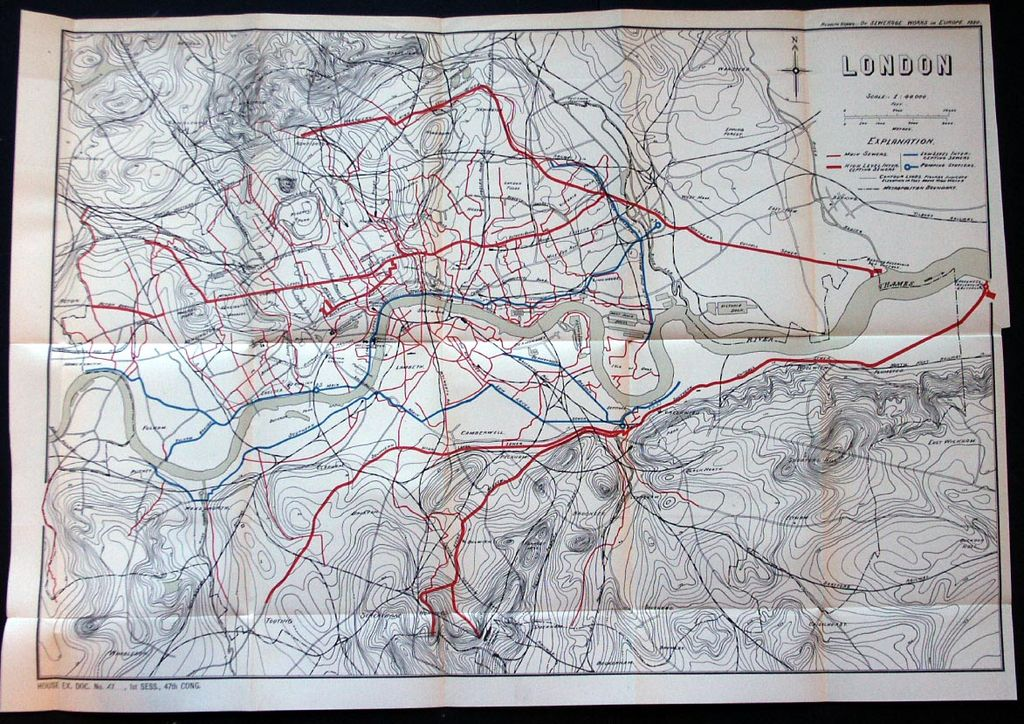
\includegraphics[width=1\textwidth]{2-cap1/complementos/mapas/1882-bazalgette-sistemadeesgotolondrino.eps}{\par \footnotesize \textbf{Fonte:} Wikipédia. \par}
\label{fig:esgotoslondres1882} 
\caption{Sistema de esgotos londrino, de construção coordenada por Joseph Bazalgette.}
\end{figure}

Entre uma epidemia e outra, um pesquisador assistente da \textit{Metropolitan Comission of Sewers}, \textit{Joseph William Bazalgette}, foi nomeado em 1856 diretor do órgão que veio a sucedê-la, o \textit{Metropolitan Board of Works}, e lá ficou até 1889; neste cargo, Bazalgette viveu em julho e agosto de 1858 -- como todos os londrinos -- o \textit{Grande Fedor}, causado pela exacerbação, pelo calor da época, do cheiro dos excrementos humanos não tratados e dos efluentes industriais que então eram lançados diretamente no Tâmisa. No mesmo ano, Bazalgette conseguiu aprovar junto ao Parlamento a construção, em Londres, de 132km de largas manilhas e canais em pedra para interceptar o afluxo de esgoto, e 1.800km de esgotamento de rua para captar os dejetos que, até então, fluiam livremente pelas ruas e vias públicas londrinas. Este fluxo de dejetos foi canalisado a jusante do Tâmisa, onde era despejado ainda sem tratamento. O plano de Bazalgette envolveu estações de bombeamento em \textit{Deptford Creek} e \textit{Crossness Point}, nos brejos de \textit{Erith}, todos no lado sul do Tâmisa; em \textit{Abbey Mills}, no vale do rio \textit{Lea}; e no aterro de \textit{Chelsea}, perto da ponte \textit{Grosvenor}, ao norte do Tâmisa \cite{bazalgette_london_1865, bazalgette_metropolitan_1865}. Embora Bazalgette fosse também adepto da teoria miasmática e pensasse, muito sinceramente, que a enorme obra sanitária que dirigiu serviria para acabar com os ``maus odores'' e, consequentemente, com as doenças epidêmicas, seus esforços tiveram sucesso, de fato, mas por um curioso efeito adverso: alargar a rede de esgotamento sanitário domiciliar e a drenagem pluvial significava conter, isolar e afastar do meio humano o bacilo do cólera, malgrado os miasmáticos duvidarem de sua existência.

\begin{figure}[!htp]
\centering
\subfloat[Claude-Philibert Barthelot, conde de Rambuteau. \textbf{Fonte:} Wikipédia.]{
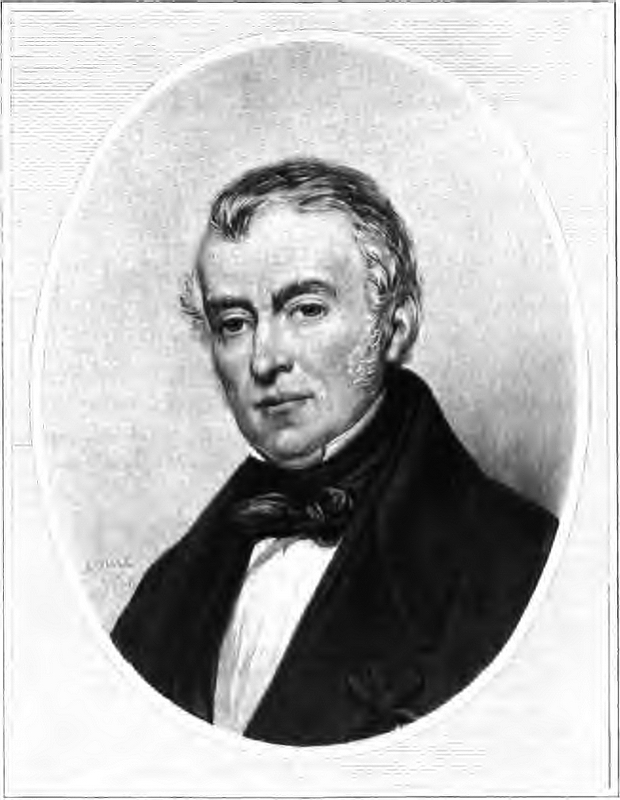
\includegraphics[width=0.4\textwidth]{2-cap1/complementos/fotos/Rambuteau.eps}
\label{fig:rambuteau}
}
\  %espaco separador
\subfloat[Georges Eugène Haussmann. \textbf{Fonte:} Wikipédia.]{
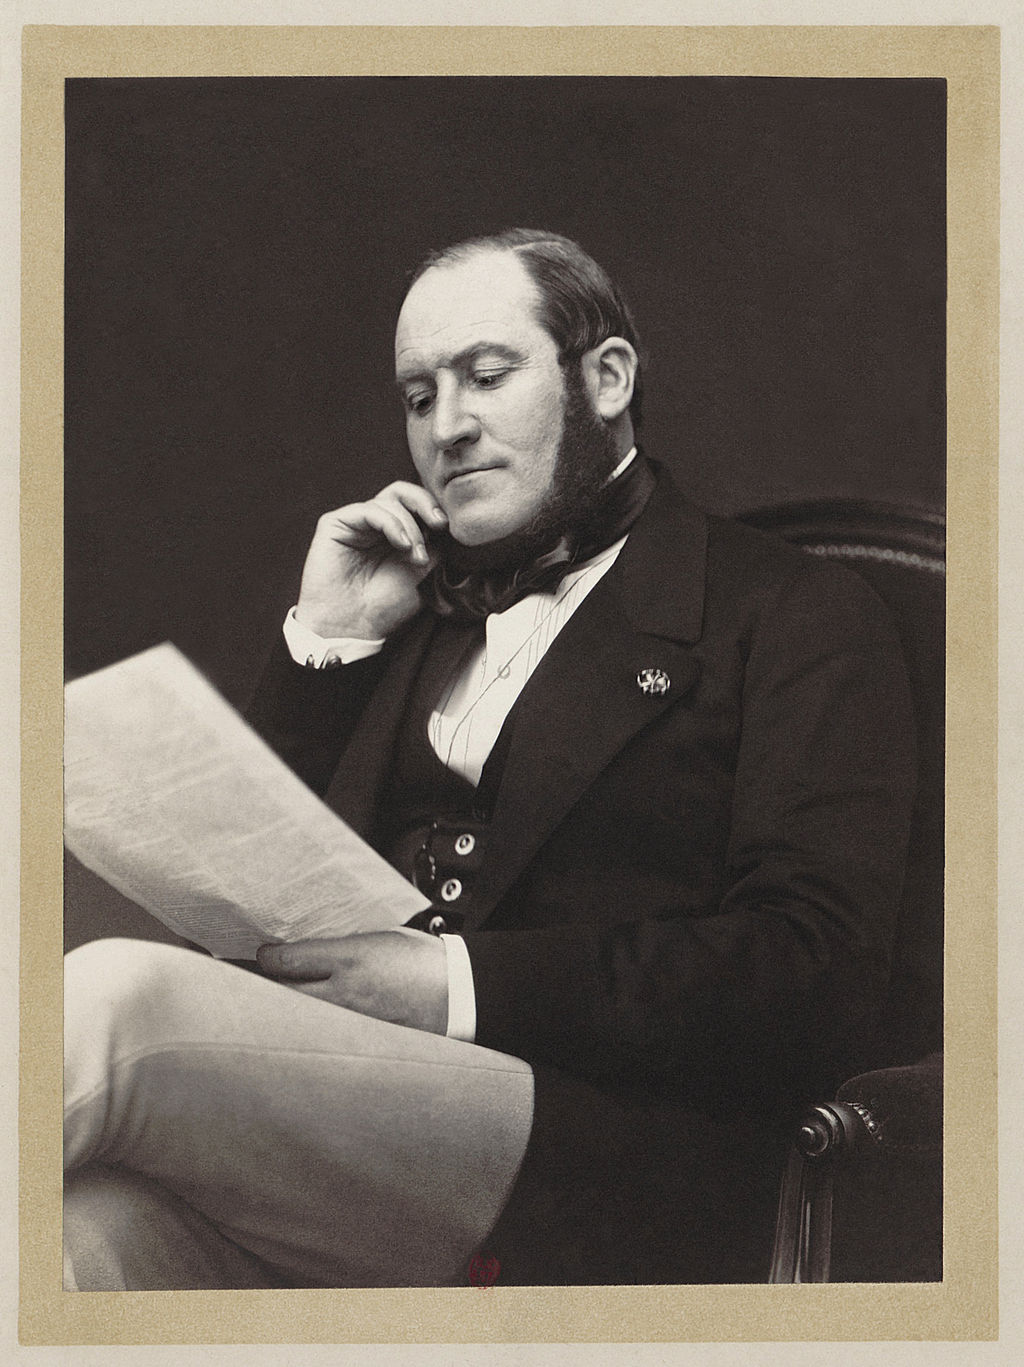
\includegraphics[width=0.4\textwidth]{2-cap1/complementos/fotos/haussmann.eps}
\label{fig:haussmann}
}
\caption{Rambuteau e Haussmann, pioneiros do urbanismo e do planejamento urbano na França.}
\end{figure}

Vejamos agora a correlação entre teoria miasmática e obras públicas em \textit{Paris}. A ideia de realizar profundas reformas no centro de Paris era tão antigo e recorrente, sob diferentes formatos e nomes, que antecedeu ao Haussmann prefeito, e que poderia, inclusive, ter sido feito inclusive sem ele. A cidade, quando de sua epidemia de cólera em 1832, havia crescido rumo aos \textit{faubourgs} em torno dos bulevares de Luís XIV, construídos em substituição às suas antigas muralhas; o centro mantinha as características medievais (principalmente as ruas estreitas e a malha viária irregular) e era dominado por uma encarniçada classe de proprietários, ciosa de seus direitos e pronta a defendê-los em qualquer instância onde se fizesse necessário \cite{faure_paris_2004}. Em 1833 \textit{Claude-Philibert Barthelot, conde de Rambuteau} foi posto à frente da prefeitura do Sena, onde permaneceu até 1848. Considerou ser seu dever ``dar aos parisienses água, ar e sombra'' \cite[p.~269]{rambuteau1905memoires}, comprimidos que eram pelas ruas estreitas e apertadas da cidade medieval; Rambuteau via-se no Hôtel de Ville como um ``comandante numa cidadela'' \cite[p.~269]{rambuteau1905memoires}, e assim tentou agir. A epidemia de cólera que assolou Paris em 1832 serviu a Rambuteau para dar início a um programa de melhoramentos urbanos iniciados com a abertura da \textit{Rue de Chanvreire} (atual \textit{Rue Rambuteau}), em 1834, com largura de 13 metros (incomum para os padrões da época), ligando o \textit{Marais} a \textit{Les Halles}; foi também aberta a \textit{Rue d'Arcole}, que atravessava a \textit{Île de la Cité} desde o arco da catedral de \textit{Notre-Dame} até o \textit{Hôtel de Ville} (ambos reformados, e o último ampliado, durante a gestão de Rambuteau); outras 112 ruas foram abertas. Seguiu-se a generalização da iluminação a gás em Paris, deixando Rambuteau ao sair de seu cargo 8.600 lampiões instalados; a rede de esgoto parisiense foi modernizada; novas pontes sobre o Sena foram construídas, sendo as mais famosas as de \textit{Bercy}, \textit{Saint-Pères} e Luís Felipe; a ilha de \textit{Louviers} foi anexada à margem direita do Sena por meio de um aterro. Rambuteau, ainda perseguindo seu programa de ``água, ar e sombra'', mandou plantar milhares de árvores e podar as já existentes; supervisionou a proliferação das ruas convexas, separadas das calçadas por sarjetas de escoamento, em substituição às antigas ruas côncavas em que as águas servidas acumulavam-se em poças; trouxe a Paris a pavimentação asfáltica, inicialmente ao redor do \textit{Palais-Royal}; ordenou a perfuração de poços em \textit{Grenele} e a instalação de duas mil fontes públicas com água encanada; a nota cômica deste processo de renovação urbana é o fato de os mictórios públicos instalados espaçadamente nos logradouros neste período terem sido apelidados de \textit{rambuteaux} em sua ``homenagem'' (\citeauthor{combeau_paris_2011}, \citeyear{combeau_paris_2011}, pp.~71-73; \citeauthor{rambuteau1905memoires}, \citeyear{rambuteau1905memoires}, pp.~325-399; \citeauthor{petti_eurfranba_2011}, \citeyear{petti_eurfranba_2011}, pp.~73-74). Em sua própria opinião, o conde de Rambuteau não pensa ter falhado em sua tarefa, pois teria feito o possível dentro das limitações legais e, no fim das contas, deixou a prefeitura do Sena sem dívidas \cite[p.~399]{rambuteau1905memoires}. 

O programa higienista concretizado primeiramente sob a gestão de Rambuteau foi retomado em escala monumental entre 1853 e 1870 por \textit{Georges Eugène Haussmann} em seu mandato à frente da prefeitura do Sena. Recentes descobertas arquivísticas demonstram que a participação de Haussmann na concepção geral das reformas no centro de Paris, ao contrário do que ele dá a entender em suas memórias (\citeauthor{haussmann1890memoires-1}, \citeyear{haussmann1890memoires-1}, \citeyear{haussmann1890memoires-2}, \citeyear{haussmann1890memoires-3}), foi menor do que se pensa: a \textit{Commission des embellissements de Paris}, nomeada diretamente por Napoleão III, composta por topógrafos, engenheiros e profissionais correlatos (como \textit{Théodore Jacoubet}, \textit{Hippolyte Meynadier} e os irmãos \textit{Louis} e \textit{Félix Lazaire}), reuniu-se pela primeira vez em 16 de agosto de 1853 e trabalhou até que seu diretor, \textit{Henri Siméon}, entregou ao imperador em 27 de dezembro de 1853 um plano bastante completo das modificações a serem feitas em Paris; muitas delas foram discutidas entre Napoleão III e a \textit{Comission} sem que Haussmann sequer tomasse parte; foi o plano resultante dos trabalhos da \textit{Comission}, com algumas alterações, que Haussmann implementou durante sua gestão à frente da prefeitura do Sena, depois de haver pedido -- e conseguido -- a extinção da comissão \cite{bourillon_changer_1999,casselle_embel_1997}\footnote{O artigo pioneiro de \citeonline{casselle_embel_1997}, quem primeiro divulgou a existência deste plano, chega a comparar, uma a uma, todas as obras propostas pela \textit{Comission} com aquelas realizadas por Haussmann ou por seus sucessores. Observa, adicionalmente, que a cidade inteira foi coberta pelo projeto original (enquanto Haussmann trabalhou principalmente na sua parte oeste), e que a malha viária dos antigos subúrbios anexados em 1860 estava, também, já desenhada no plano da \textit{Comission} de 1853, como a indicar um plano concebido de antemão.}. Quer como mentor intelectual, quer como gestor a mão-de-ferro de planos pré-concebidos, as obras regidas por Haussmann, ao contrário daquelas regidas por Rambuteau, são muito maiores em escala e número, e muito mais conhecidas e comentadas \cite{bourillon_changer_1999, casselle_embel_1997, dansette_haussmann_1972, faure_paris_2004, hourticq_haussmann_1971, petti_eurfranba_2011, pinkney_ordevpar_1955, pinkney_paris_1957, vossen_villes_1947}, sendo desnecessário para o objeto desta pesquisa detalhá-las neste momento; cabe, muito mais, ressaltar que Haussmann era outro adepto da teoria miasmática (\citeauthor{haussmann1890memoires-2}, \citeyear{haussmann1890memoires-2}, p.~318; \citeyear{haussmann1890memoires-3}, p.~421), e que a orientação geral das intervenções urbanas regidas por seus planos seguia, mesmo que não intencionalmente, o programa de Rambuteau e de outros predecessores (Chabrol, Berger, o ``plano dos artistas'', os largos \textit{boulevards} à moda de Luís XIV etc.). Num só e grande resumo:

\begin{citacao}
Mas, afinal, o que é haussmannização? Através dos escritos de Haussmann, não se pode chegar a um conceito preciso, uma vez que ele não propõe uma doutrina ou uma teoria de melhorias urbanas.
[\dots] O próprio Haussmann chama seu trabalho de regularização, que não pretende uma universalidade científica, não se baseia numa crítica social, nem propõe um modelo espacial.
[\dots] As intervenções haussmannianas mudam a maneira de pensar a cidade, tomando como principal elemento a rua e criando uma rede viária composta por um tecido arquitetônico que destrói bairros insalubres e vielas. Expulsam a população residente, melhoram a higiene e a circulação, mudam a imagem da área central, e a cidade prepara-se para um novo modo de vida. A rua do século XIX destrói e modifica a rua medieval. A caixa da rua aumenta, as fachadas são reconstruídas, os trechos irregulares são substituídos por outros com desenho regular, geométrico e reto. Diferentes dos bulevares de Luís XIV -- projetados no lugar das antigas muralhas, locais para o desfrute e o passeio --, os bulevares do século XIX, de Haussmann, são artérias criadas para a circulação rápida, o tráfego pesado. O espaço haussmanniano é o espaço público -- a rua, o passeio, as praças --, o espaço da mobilidade. A originalidade desse projeto está no conceito de sistema de circulação e de respiração, que superpõe malhas hierarquizadas, pertencentes a uma rede em estrela. Esse desenho não resulta num espaço homogêneo, uma vez que se acentua a divisão social entre leste e oeste, entre periferia e centro, mas ainda não se adota a ideia de cidade por setores. A hierarquia do sistema de comunicações muda a ordem de valores.
[\dots] Na cidade haussmanniana, é introduzida uam nova forma de construção da paisagem urbana. As intervenções no núcleo central tratam o conjunto dos espaços heterogêneos como uma entidade única e o dotam de isotropia. Constrói-se uma imagem urbana mais coerente, com um tipo de arquitetura definida, em que o imóvel se integra no espaço público através de uma projetação regulamentada \cite[pp.~68,~77]{petti_eurfranba_2011}.
\end{citacao}

A saúde pública e o bem-estar dos cidadãos parisienses era o principal argumento para a instalação, reforma ou ampliação de infraestruturas sanitárias e equipamentos coletivos, mas não era possível esconder os profundos arranjos financeiros necessários a tais reformas: a oposição parlamentar a Napoleão III atacou Haussmann incessantemente pela falta de transparência nos gastos, especialmente com o escândalo das transações escusas envolvendo o \textit{Crédit Foncier}, a \textit{Caisse des Travaux de Paris} e a firma \textit{Ardoin, Ricardo et Cie.} \cite{pinkney_paris_1957}. Houve desde o início das intervenções resistência encarniçada ao programa de reformas também entre proprietários, que julgavam indevidas as expropriações e as intervenções sobre suas propriedades \cite{paccoud_hauspropr_2012}. A força combinada destas pressões políticas levou Napoleão III a retirar o apoio a Haussmann, que saiu da prefeitura do Sena em 1870. Não obstante, as reformas ditas ``haussmannianas'' (mais bem descritas como \textit{reformas do Segundo Império}), numa Paris cujo centro estava sendo progressivamente abandonado pelas classes abastadas e ocupado pelos trabalhadores e pelos miseráveis, cujos alugueis abasteciam os bolsos dos proprietários fundiários, teria beneficiado exatamente os mais abastados, já em vias de instalação nos \textit{faubourgs} e subúrbios parisienses, a obter vantagens na luta encarniçada pela retomada do centro de Paris \cite{faure_paris_2004}.

\begin{figure}[!htp]
\centering
\subfloat[Abertura da \textit{Avenue de l'Ópera}. \textbf{Fonte:} Wikipédia.]{
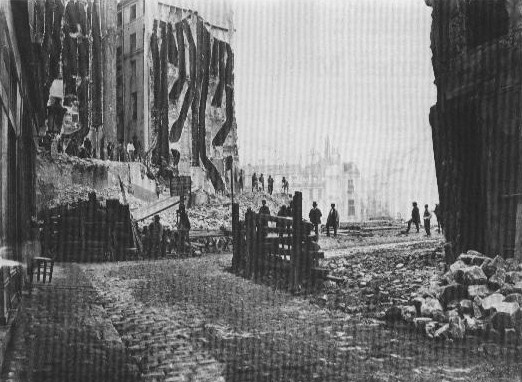
\includegraphics[width=1\textwidth]{2-cap1/complementos/fotos/Percement_avenue_de_lOpera.eps}
\label{fig:aberturaopera}
}
\  %espaco separador
\subfloat[Trabalhos noturnos de construção da \textit{Rue de Rivoli} iluminados por luz elétrica. \textbf{Fonte:} Wikipédia.]{
\includegraphics[width=1\textwidth]{2-cap1/complementos/fotos/rivoli.eps}
\label{fig:obrasrivoli}
}
\caption{Obras do período de Georges Eugène Haussmann à frente da prefeitura do Sena.}
\end{figure}

A análise de exemplos poderia incluir a construção em Viena (Áustria) da \textit{Ringstrasse} e seus prédios monumentais por ordem do imperador Francisco José I (1857-1913) \cite{abercrombie_vienna_1910,abercrombie_vienna_1911,aman_vienna_1911}; poderia incluir o ``embelezamento'' de Bruxelas (Bélgica) sob a regência do burgomestre \textit{Jules Anspach} e do rei \textit{Leopoldo II} (\textit{le roi bâtisseur}, ``o rei construtor''), em especial o tamponamento e canalização do Sena entre 1859 e 1873 \cite{abercrombie_brussels1_1912,abercrombie_brussels2_1912,abercrombie_brussels3_1913}; poderia avançar pela expansão de Barcelona de acordo com o plano pioneiro de \textit{Ildefonso Cerdà} (1860) \cite{aibarbijker_barcelona_1997,ciervo_cerda_1976,soriaypuig_cerda_1995,wynn_barcelona_1979}; poderia seguir pelo \textit{Risanamento} de Florença (1865-1895), Nápoles (1885-1904) e outras cidades italianas em seguida à \textit{Unificazione} \cite{biocca_naples_1992,parisi_napoli_2001,piccinato_igiene_1989,rossi_napoli_2011}\dots Há um longo fio condutor a ligar o higienismo dos primeiro e segundo terços do século XIX ao ``proto-urbanismo'' do último terço deste mesmo século e ao urbanismo do primeiro terço do seguinte -- se é que há, realmente, alguma solução de continuidade, salvo pela escala e escopo das intervenções propostas em ambos os casos. 

\begin{figure}[!htp]
\centering
\includegraphics[width=1\textwidth]{2-cap1/complementos/mapas/1856_Bauplanungen.eps}{\par \footnotesize \textbf{Fonte:} Wikipédia. \par}
\label{fig:bauplannungen1856} 
\caption{Planta de situação da capital e da cidade residencial de Berlim e seus arredores -- plano de desenvolvimento dos arredores de Berlim (1856).}
\end{figure}

\begin{figure}[!htp]
\centering
\includegraphics[width=1\textwidth]{2-cap1/complementos/mapas/Boehm_Berlin_1862.eps}{\par \footnotesize \textbf{Fonte:} Wikipédia. Os 14 departamentos do plano Hobrecht estão rotulados como algarismos romanos. Os assentamentos programados estão indicados por letras maiúsculas e ruas por meio de algarismos arábicos, cada um dentro de um departamento de planejamento. \par}
\label{fig:berlin1862} 
\caption{Plano de Berlim e arredores até Charlottenburg: mapa do plano de desenvolvimento dos arredores de Berlim (1862).}
\end{figure}

\begin{figure}[!htp]
\centering
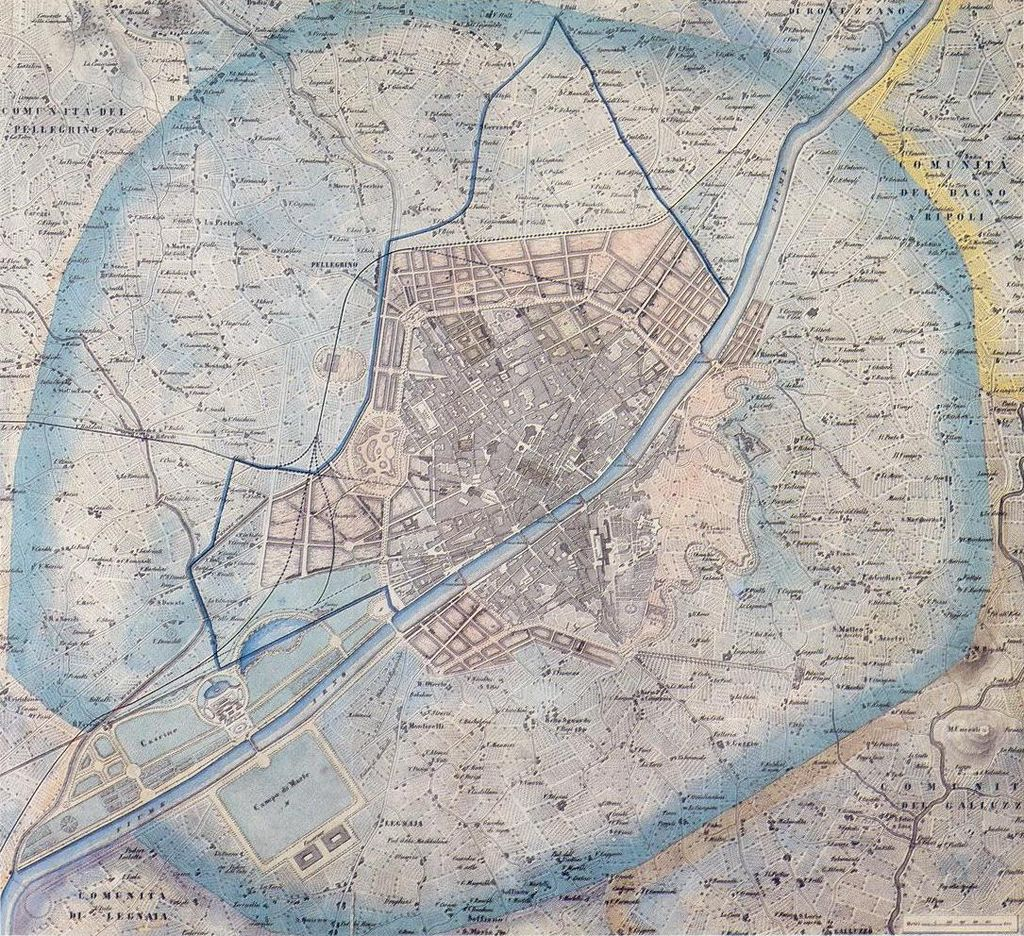
\includegraphics[width=1\textwidth]{2-cap1/complementos/mapas/1865-planopoggi-florenca.eps}{\par \footnotesize \textbf{Fonte:} Wikipédia. \par}
\label{fig:florenca1865} 
\caption{Plano de Giuseppe Poggi para Florença (1865).}
\end{figure}

\begin{figure}[!htp]
\centering
\includegraphics[width=1\textwidth]{2-cap1/complementos/mapas/heilbronn.eps}{\par \footnotesize \textbf{Fonte:} Wikipédia. \par}
\label{fig:heilbronn1879} 
\caption{Plano da cidade de Heilbronn, por Reinhardt Baumeister (1879).}
\end{figure}

Para os fins desta pesquisa, entretanto, os dois casos paradigmáticos apresentados já demonstram, sem necessidade de análise detalhada de outros exemplos, que o alvo preferencial das políticas do higienismo no século XIX foram os \textit{centros urbanos ditos ``degradados''} e as \textit{construções insalubres}. Ora, mas \textit{quem morava em tais construções e centros era exatamente quem não tinha condições de pagar para morar em imóveis em condições mais higiênicas}; ``higienizar'', ``embelezar'', fazer ``melhoramentos'' implicou, na maioria dos casos, em \textit{processos maciços de remoção dos trabalhadores e dos mais pobres dos bairros centrais}\footnote{No caso francês, \citeonline[p.~445]{faure_paris_2004} registra que ``dos 102 imóveis construidos nos anos 1860 pela companhia imobiliária dos irmãos Péreire, no atual bulevar Voltaire -- ou seja, num \textit{faubourg} do leste de Paris -- apenas 19\% dos apartamentos, dado o valor dos alugueis, parecem, a rigor, acessíveis a famílias operárias, a menos que se trate de cubículos nos sótãos''. Diz ainda que ``as operações de 1849-1853 tiveram como efeito desalojar 9.081 'trabalhadores' [\dots]: 2,1\% partiram para os \textit{banlieues}, e a imensa maioria dos outros se distribuiriam nos \textit{faubourgs}, uma reduzida minoria tendo permanecido nos bairros do centro, esperando, sem dúvida, que a continuação das obras não lhes desse caça'' (\Ibidem[p.~445]{faure_paris_2004}). No caso napolitano, tanto antes quanto depois do \textit{Risanamento} \citeonline{serao1906ventre} denunciou o caráter deletério das condições de vida dos trabalhadores mais pobres. No caso vienense, a \textit{Ringstrasse} acentuou a segregação socioespacial já existente, separando os burgueses da nova e resplandescente avenida, os operários dos subúrbios industriais como \textit{Ottakring} e uma pequena burguesia saudosa da antiga cidade \cite[p.~26]{maderthanermuser_vienna_2003}.}. O longo experimento higienista do século XIX interferiu também sobre a moradia, em especial sobre a moradia dos trabalhadores. A \textit{habitação operária} tornou-se, em paralelo à questão sanitária, pauta importante para os gestores públicos e os encontros internacionais de arquitetos e engenheiros: infiltou-se no Congresso Internacional de Higiene de 1878 em Paris \cite{congres_hygiene_1878}, fato repetido nos congressos internacionais de arquitetos de Londres (1908) e Viena (1910) \cite{QUINTOJR1990}, e mereceu um congresso internacional voltado apenas ao seu debate \cite{fleming_housing_1897}. Em nenhum deles, entretanto, chegou-se a qualquer solução definitiva quanto à questão, restringindo-se tais encontros ao relato das experiências locais em habitação operária e a soluções tópicas\footnote{Veja-se, como exemplo, o voto final da sessão plenária de 7 de agosto do Congresso Internacional de Higiene de 1878: depois de longos relatos e debates sobre a habitação dos operários em Paris, Londres, Bruxelas e outras metrópoles europeias, os presentes concordaram numa única recomendação: reforçar a legislação urbanística existente e transformar em exigência legal a instalação de água nas casas para operários \cite[p.~597]{congres_hygiene_1878}.}.

Tudo indica, até o momento, que os conflitos sociais são elemento essencial da produção, apropriação e uso dos territórios urbanos no período. Mas se há conflito social neste âmbito, seria a estética arquitetônica, ela própria, também produto dos conflitos sociais de seu tempo? Ou estaria imune a tal influência?

\subsubsection{As artes de morar: ecletismo e pré-modernismos, por dentro e por fora}\label{subsec:armor}

Entre os estilos arquitetônicos dezenovistas, o que mais interessa a esta pesquisa, pelo que se pôde encontrar nos documentos consultados, é como que um ``não-estilo'': o \textit{eclético}, resumidamente conceituado por um especialista como

\begin{citacao}
a cultura arquitetônica própria de uma classe burguesa que dava primazia ao conforto, amava o progresso (especialmente quando melhorava suas condições de vida), amava as novidades, mas rebaixava a produção artística e arquitetônica ao nível da moda e do gosto \cite[p.~13]{patetta_ecletismo_1987}.
\end{citacao}

A própria etimologia grega da palavra -- o adjetivo \textgreek{ἐκλεκτικός}, \textit{eklektikos}, ``escolhido entre os melhores'', por sua vez derivado de \textgreek{ἐκλεκτός}, \textit{eklektos}, ``escolhido, seleto'' -- indica uma de suas características principais: a escolha pelo arquiteto ou por seus clientes, na tradição arquitetônica passada, de elementos ora coerentes, ora díspares, que compusessem a obra de acordo com o gosto do freguês ou com a função a ser dada ao imóvel. Justo por isto, há enorme heterogeneidade estilística no campo eclético, sendo bastante difícil encontrar elementos comuns que não as justaposições e os revivalismos. 

Como movimento artístico, o ecletismo ocorre na arquitetura e na arte do século XIX. As primeiras vanguardas desse movimento datam da terceira década do século XIX com a
afirmação de pulsões neo-góticas em áreas francófonas e neo-renascentistas em Florença. Por volta de 1840, na França, em reação à hegemonia do estilo greco-romano, os arquitetos começam a propor a retomada de outros modelos históricos como, por exemplo, o gótico e o românico. O principal teórico do ecletismo arquitetônico é o francês \textit{César Denis Daly} (1811-1893) que o entende como ``o uso livre do passado''. Não se trata de uma atitude de simples copista, mas da habilidade de combinar as características superiores desses estilos em construções que satisfaçam a demandas da época por todo tipo de edificação. Na segunda metade do século XIX, o ecletismo tem forte presença na Europa. O estilo \textit{Segundo Império} ou \textit{Napoleão III} é caracterizado pela realização de importantes edifícios ecléticos, como o Teatro Ópera de Paris, projetado por \textit{Charles Garnier} (1825-1898).

\begin{figure}[!htp]
\centering
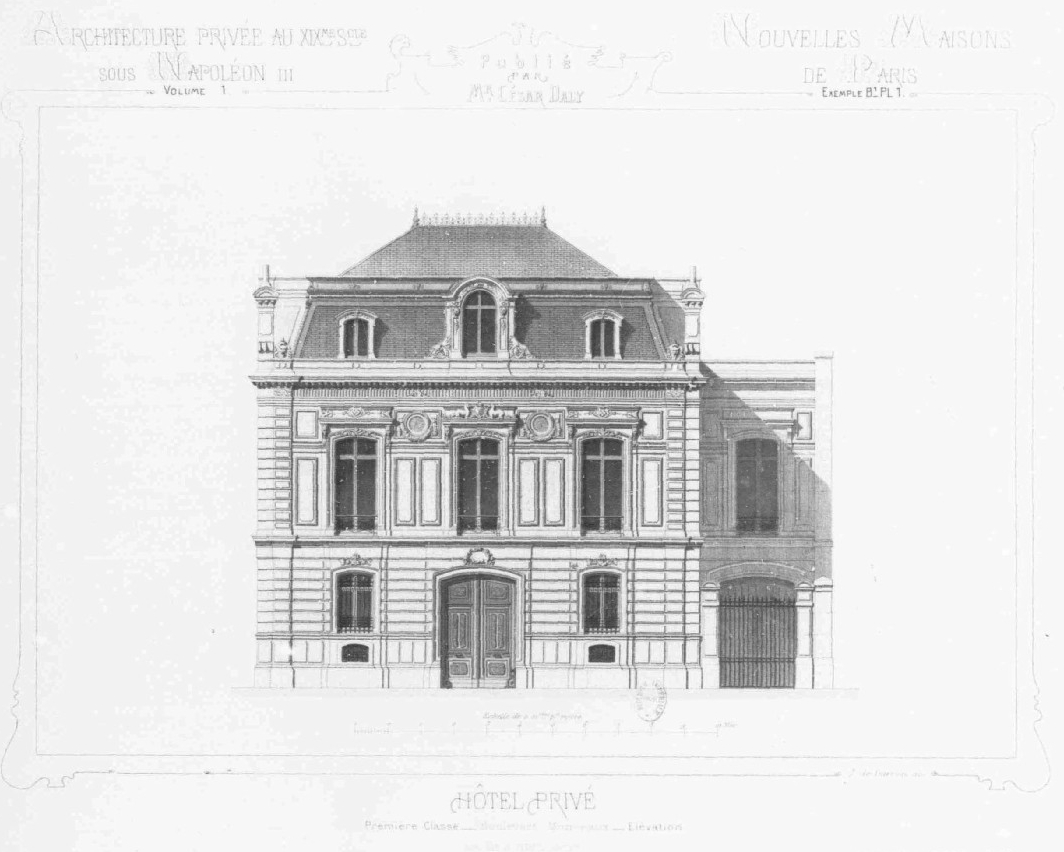
\includegraphics[width=1\textwidth]{2-cap1/complementos/fotos/daly01-0.eps}{\par \footnotesize \textbf{Fonte:} \citeonline{daly_architecture1_1864}. \par}
\label{fig:hotelprimclas} 
\caption{\textit{Hôtel privé} de primeira classe no estilo Segundo Império/Napoleão III.}
\end{figure}

\begin{figure}[!htp]
\centering
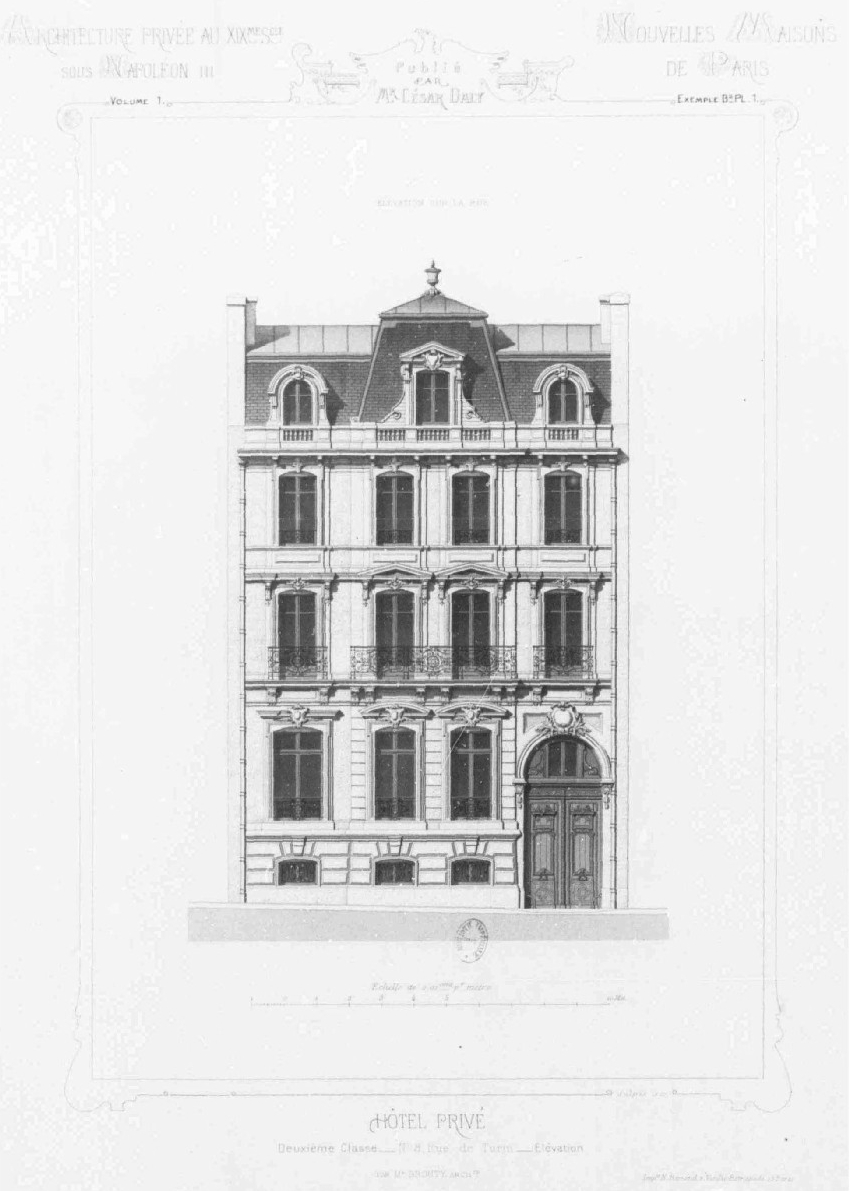
\includegraphics[width=1\textwidth]{2-cap1/complementos/fotos/daly01-1.eps}{\par \footnotesize \textbf{Fonte:} \citeonline{daly_architecture3_1864}. \par}
\label{fig:hotelsegclas} 
\caption{\textit{Hôtel privé} de segunda classe no estilo Segundo Império/Napoleão III.} 
\end{figure}

\begin{figure}[!htp]
\centering
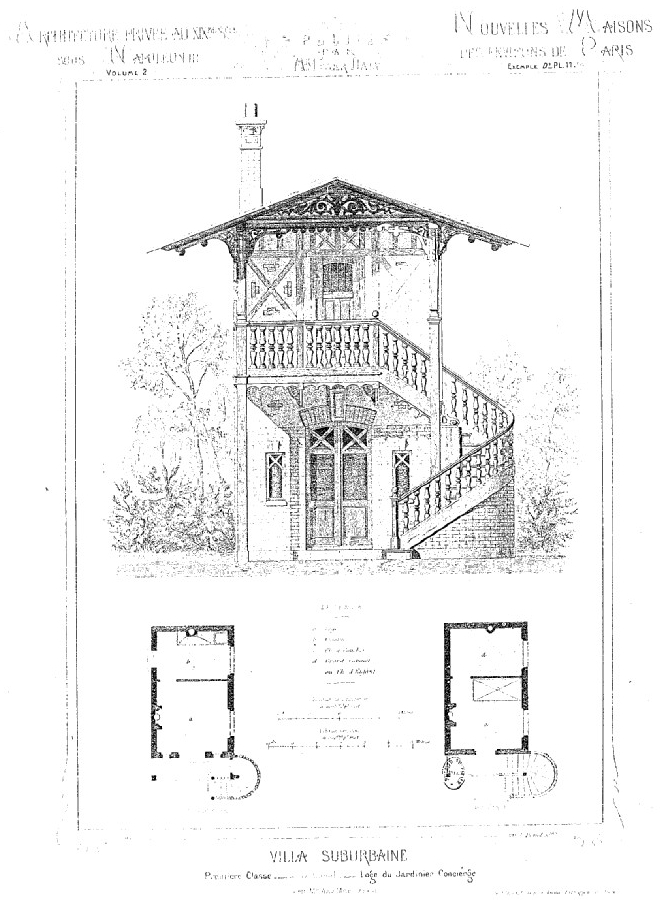
\includegraphics[width=1\textwidth]{2-cap1/complementos/fotos/daly03-4.eps}{\par \footnotesize \textbf{Fonte:} \citeonline{daly_architecture3_1864}. \par}
\label{fig:villaprimclas} 
\caption{\textit{Villa suburbaine} de primeira classe no estilo Segundo Império/Napoleão III.}
\end{figure}

\begin{figure}[!htp]
\centering
\subfloat[\textbf{Fonte:} \citeonline{daly_architecture3_1864}.]{
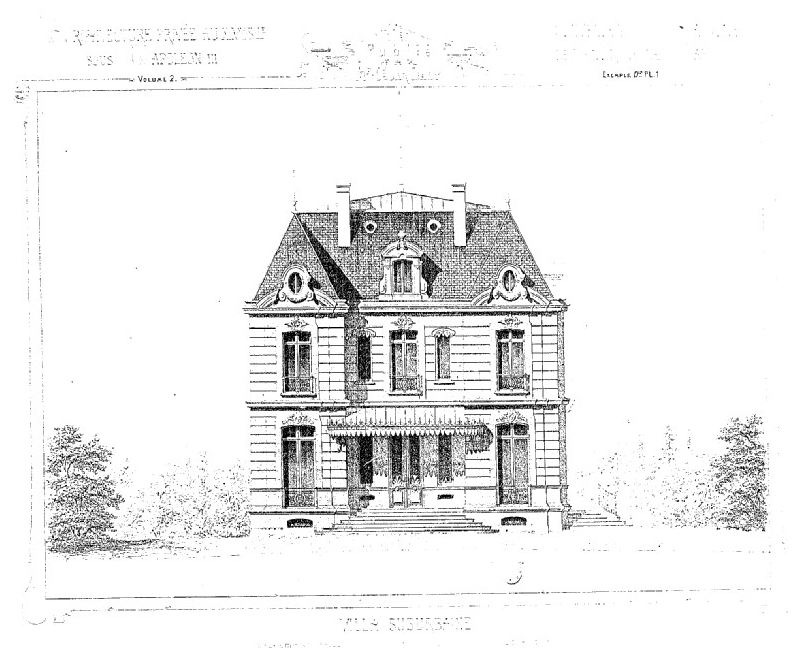
\includegraphics[width=0.9\textwidth]{2-cap1/complementos/fotos/daly03-5.eps}
\label{fig:villasegclas1}
}
\  %espaco separador
\subfloat[\textbf{Fonte:} \citeonline{daly_architecture3_1864}.]{
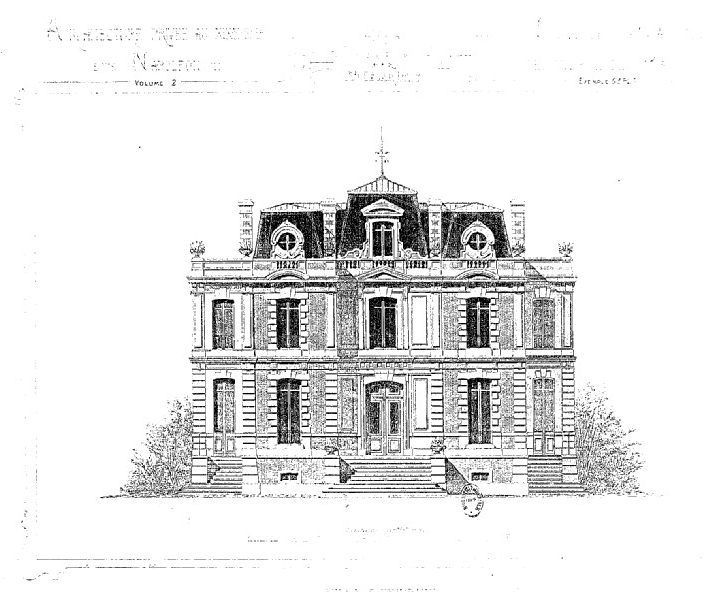
\includegraphics[width=0.9\textwidth]{2-cap1/complementos/fotos/daly03-6.eps}
\label{fig:villasegclas2}
}
\caption{\textit{Villas suburbaines} de segunda classe no estilo Segundo Império/Napoleão III.}
\end{figure}

\begin{figure}[!htp]
\centering
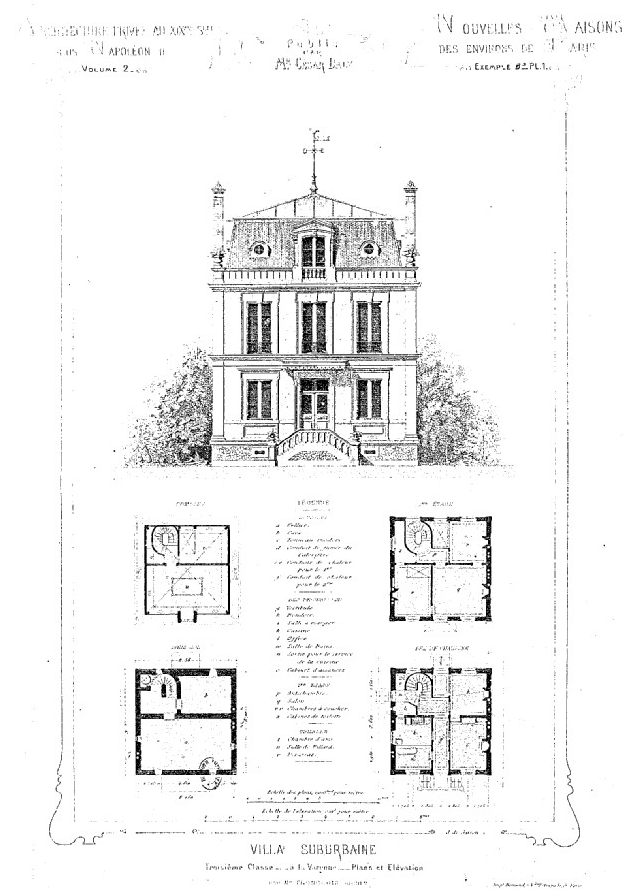
\includegraphics[width=1\textwidth]{2-cap1/complementos/fotos/daly03-8.eps}{\par \footnotesize \textbf{Fonte:} \citeonline{daly_architecture3_1864}. \par}
\label{fig:villaterclas} 
\caption{\textit{Villa suburbaine} de terceira classe no estilo Segundo Império/Napoleão III.}
\end{figure}

As diferentes linguagens artísticas foram reelaboradas a critério do arquiteto seguindo a sua inspiração pessoal. No princípio a tendência eclética se impôs especialmente na realização de estruturas para festas e grandes eventos; sucessivamente, começou a ser apreciada também para mobiliar casas e jardins, nos quais, frequentemente e de forma totalmente acrítica, misturavam-se tempos gregos, vasos árabes e pavilhões indianos. Na época afirmou-se o costume de mobiliar cada sala das residências mais luxuosas segundo um estilo diferente. Assim, marceneiros e ebanistas, por exemplo, tiveram que aprender a lidar com formas bastante diferentes entre si. 

Mas foi o modernismo industrial do século XIX que serviu como trampolim para o sucesso do estilo eclético. Em 1851, pela primeira vez, na \textit{Great Exhibition} em Londres foram realizados pavilhões onde os mercadores das principais nações do mundo foram chamados para expor suas próprias obras. Percebeu-se que as empresas presentes exibiam para a atenção do publico obras que mostravam a história recente ou antiga da própria nação. Houve euforia em expor todas as obras antigas remodeladas, havendo-se, inicialmente, um certo grau de dependência relativamente aos modelos originais, quase como se fosse uma cópia, uma reprodução. A fantasia de cada artista, artesão, arquiteto, ourives, etc. não demorou para se afirmar, levando os artistas a formular obras personalizadas que ``condensavam'' vários séculos de história. Era isso o que os clientes queriam, curiosos por artes distantes e citações culturais magníficas mostrando que aquela geração iria reviver uma era áurea. Todas as grande técnicas do passado reviviam numa miríade de moveis, cerâmicas e
objetos do Ecletismo.

Grosso modo, as obras arquitetônicas em estilo eclético podem ser classificadas em três categorias principais, cujas características são assim definidas:

\begin{itemize}
\item A \textit{composição estilística}: caracteriza-se por um \textit{maior rigor filológico} e pela \textit{imitação precisa e coerente de um único e preciso estilo arquitetônico}. Os exemplos mais destacados são o \textit{neogrego}, o \textit{neo-egípcio} e o \textit{neogótico}.
\item O \textit{historicismo tipológico}: caracteriza-se por uma \textit{relação apriorística de cunho analógico entre estilo e função} através de valores associativos, não raro arbitrários. A arquitetura medieval, por exemplo, forneceu aos arquitetos os traços místicos e a religiosidade para as novas igrejas; na arquitetura renascentista foram encontradas as características áulicas elegantes para os edifícios públicos; na arquitetura barroca, ou nos estilos orientais, a festividade exigida pelos equipamentos; no classicismo pesado do coríntio romano, o caráter apropriado aos solenes edificios parlamentares, aos museus e aos ministérios.
\item Os \textit{pastiches compositivos}: caracterizam-se pela \textit{fusão de elementos arquitetônicos de estilos distintos, historicamente inadmissíveis}, sob cujos elementos díspares, não raro beirando o mau gosto, mascaravam-se muitas vezes soluções estruturais inovadoras \cite[p.~14-15]{patetta_ecletismo_1987}.
\end{itemize}

Quer seja ele o estilo ostentatório dos \textit{nouveaux riches} desprovidos da bagagem cultural do \textit{Ancièn Régime} e dispostos a demarcar seu espaço social por meio da sobreposição, às vezes sem nexo, das novas modas da Escola de Belas-Artes de Paris \cite[pp.~315-319]{guerrand_espacos_2009}, quer seja um estilo arquitetônico com méritos e conquistas próprios em processo de redescoberta desde pelo menos a metade dos anos 1970, a partir da crítica ao ideário arquitetônico do Modernismo que o sucedeu e criticou duramente \cite{almeida_victoria_1997, almeida_vitrinescomercio_2014, patetta_ecletismo_1987, puppi_hisnamod_1998}, interessa a esta pesquisa o fato de o ecletismo ser o estilo arquitetônico mais encontrado no distrito soteropolitano estudado, especialmente nas modalidades de \textit{historicismo tipológico} e \textit{pastiche compositivo}, com maior frequência esta última.

A América Latina foi terreno fértil para as experimentações arquitetônicas, especialmente as ecléticas, e isto por questões muito particulares. No final do século XIX, findos os processos independentistas, consolidadas as fronteiras nacionais e assentados os blocos hegemônicos na política após um século pontilhado por guerras, \textit{pronunciamientos} e rebeliões, as classes dominantes nos países latinoamericanos viram na arquitetura um meio de reafirmar sua identidade nacional. Curiosa e paradoxalmente, entretanto, tal como em outros campos da cultura, esta reafirmação se deu por meio de símbolos e elementos tomados de empréstimo por estas mesmas classes dominantes às edificações da aristocracia, dos banqueiros, dos grandes comerciantes e industriais da Europa \cite[pp.~403-406]{gutierrez_arquibero_1983}. Conquanto haja leitura destes empréstimos no sentido de criar uma clivagem entre colonizados e colonizadores, em que os primeiros -- como um todo, sem qualquer clivagem, estruturação, estratificação ou hierarquização social internas a si próprios -- encontrar-se-iam sempre no encalço destes últimos por quaisquer razões \cite{bhabha_local_1998,memmi_coloniza_1967}, na perspectiva adotada por esta pesquisa parece mais plausível radicar estes empréstimos nos deslocamentos miméticos de ideias e práticas devido à \textit{inserção subordinada destas classes dominantes no capitalismo internacional e no colonialismo} \cite{schwarz_ideias_1973}. As duas correntes, entretanto, concordam em que o deslocamento de ideias, símbolos e signos de seu contexto original produz efeitos bastante diversos no novo contexto em que se inserem, e que são eles, e não aqueles produzidos em seu ambiente de origem, que devem ser estudados. Esta ``chave de leitura'' será importante para a análise da urbanização brasileira na Primeira República, mais adiante.

E aqui, nesta etapa pré-modernista do pensamento e da prática acerca das cidades, se encerram as condicionantes sincrônicas internacionais relevantes para a presente pesquisa. As defasagens entre a produção e circulação de ideias nos meios profissonais levam a que as primeiras influências da arquitetura e do urbanismo europeus de vanguarda surgidas entre a última década do século XIX e as duas primeiras décadas do século XX, em seu pensamento ou realizações, só se façam sentir sobre o pensamento e a prática da arquitetura e do urbanismo em Salvador nos trabalhos da Semana de Urbanismo de 1935, que extrapolam o limite temporal escolhido\footnote{É certo, por exemplo, que Theodoro Sampaio mencionou explicitamente a influência sobre ele exercida pelas cidades-jardim \cite{costa1996theodoro}, e que já em 1913 estas mesmas cidades-jardins eram debatidas na imprensa baiana como contraponto ao desleixo da administração pública com o problema das moradias populares \cite{flexor_salvadorverde_2000}; apesar disto, nem o projeto da Cidade da Luz foi adiante (sua implementação em 1937 se deu vinte e oito anos depois da apresentação do projeto original de Theodoro Sampaio), nem os debates na imprensa avançaram além do confronto de ideias.}.